% main_4.tex - C4-Den-Mat on PriMock57 uses LOO PriMock57 (same as C3-Lex-Mat); Table~1 and narrative updated; aligned with eval_57 and verify_thesis_facts.py.
\documentclass[11pt,a4paper,twocolumn]{article}

\usepackage[margin=1.7cm, top=2.0cm, bottom=2.3cm]{geometry}
\usepackage[T1]{fontenc}
\usepackage[utf8]{inputenc}
\usepackage[british]{babel}
\usepackage{newtxtext,newtxmath}
\usepackage{graphicx}
\graphicspath{{./}{images/}{../images/}{../thesis/}{../thesis/images/}}
\usepackage{subcaption}
\usepackage{booktabs}
\usepackage{tabularx}
\usepackage{multirow}
\usepackage{array}
\usepackage{xcolor}
\usepackage{colortbl}
\usepackage{amsmath}
\usepackage{float}
\usepackage{caption}
\usepackage{setspace}
\usepackage{parskip}
\usepackage{enumitem}
\usepackage{titlesec}
\usepackage{microtype}
\usepackage{fancyhdr}
\usepackage{tcolorbox}
\usepackage{abstract}
\usepackage{stfloats}
\usepackage{ragged2e}
\let\Bbbk\relax
\usepackage{amssymb}
\usepackage{placeins}
\usepackage{cite}
\usepackage{hyperref}
\hypersetup{colorlinks=true, linkcolor=black, citecolor=black, urlcolor=black}

\definecolor{siggreen}{HTML}{D6EAD6}
\definecolor{sigunsig}{HTML}{FAD7D7}
\definecolor{lightgray}{HTML}{F5F5F5}
\definecolor{medgray}{HTML}{CCCCCC}

\titleformat{\section}{\normalsize\bfseries}{\thesection}{1em}{}
\titleformat{\subsection}{\normalsize\bfseries}{\thesubsection}{1em}{}
\titleformat{\subsubsection}{\normalsize\itshape}{\thesubsubsection}{1em}{}
\titlespacing{\section}{0pt}{8pt}{3pt}
\titlespacing{\subsection}{0pt}{6pt}{2pt}
\titlespacing{\subsubsection}{0pt}{5pt}{2pt}

\renewcommand{\abstractnamefont}{\normalsize\bfseries}
\renewcommand{\abstracttextfont}{\normalsize}
\renewcommand{\abstractname}{Abstract\par\vspace{6pt}}
\setlength{\absleftindent}{0pt}
\setlength{\absrightindent}{0pt}

\setlength{\parskip}{2pt}
\setlength{\parindent}{0pt}
\setlength{\columnsep}{0.6cm}

\captionsetup{font=small, labelfont=bf, skip=4pt, width=0.95\linewidth}

\newcommand{\up}{\textcolor{green!60!black}{$\uparrow$}}
\newcommand{\dn}{\textcolor{red!70!black}{$\downarrow$}}
\newcommand{\best}{\checkmark}
\newcommand{\bestnum}[1]{\textbf{#1}}
\newcommand{\fnmark}[1]{\textsuperscript{#1}}

\tcbuselibrary{skins,breakable}
\newtcolorbox{notebox}{
  colback=lightgray, colframe=medgray,
  boxrule=0.5pt, arc=3pt,
  left=5pt, right=5pt, top=4pt, bottom=4pt,
  breakable, fontupper=\small
}

\pagestyle{fancy}
\fancyhf{}
\fancyhead[C]{\small\textit{Retrieval-Augmented Reformulation for Improving Noisy ASR Transcripts}}
\fancyfoot[C]{\thepage}
\renewcommand{\headrulewidth}{0.4pt}

% Avoid bad hyphenation (e.g. re-trieval)
\hyphenation{retrieval}

\begin{document}

\twocolumn[{%
\begin{center}
  {\Large\bfseries Retrieval-Augmented Reformulation\\[4pt]
  for Improving Noisy ASR Transcripts}\\[10pt]
  {\normalsize Darragh Kerins}\\[2pt]
  {\normalsize University of the Basque Country (UPV/EHU)\quad|\quad
               MSc Language Analysis \& Processing}
\end{center}
\vspace{6pt}
\hrule height 0.5pt
\vspace{6pt}
\begin{abstract}
\setstretch{1.03}
Automatic speech recognition (ASR) transcripts often contain lexical and
semantic errors that degrade downstream usability. Retrieval-augmented
generation (RAG) has been proposed as a post-processing approach that
grounds a language model in external passages to improve transcript quality.
This work evaluates lexical and dense RAG reformulation pipelines for ASR
correction across three datasets: TED-LIUM, MTS-Dialog, and PriMock57
clinical consultations. Experiments compare generic and domain-matched
retrieval using BM25 and dense embeddings with a Mistral-7B generator in a
$2{\times}3$ design over retrieval modality and corpus scope.
Results show that dense retrieval substantially improves WER on clean
TED-LIUM transcripts, reducing WER by up to 54\% relative to an LLM-only
baseline, while generic lexical RAG can degrade performance. On clinical
data, however, domain-matched retrieval frequently degrades biomedical
entity fidelity (DISEASE~F1, $p < 0.01$) even when semantic metrics such as
BERTScore remain stable. These findings highlight a \textbf{clinical corpus
penalty}: retrieval grounding can introduce plausible but incorrect domain
entities, suggesting that entity-aware retrieval or stronger constraints are
required for safe clinical deployment.
\end{abstract}
\vspace{6pt}
\hrule height 0.5pt
\vspace{8pt}
}]

\section{Introduction}

ASR models such as Whisper still fail in challenging conditions: accented
speech, background noise, and domain-specific vocabulary. In clinical settings
the stakes are concrete: \textit{lisinopril} transcribed as \textit{listen oh
pill} can propagate into a clinical note and affect downstream care.

LLM-based post-correction is one remedy, but LLMs tend to paraphrase rather
than minimally correct, which harms lexical fidelity. Retrieval-Augmented
Generation (RAG) grounds the LLM in external passages. As this paper shows,
retrieving from the wrong corpus introduces a worse problem: entity
substitutions that look semantically correct but are clinically wrong, and
invisible to BERTScore.

This paper evaluates RAG post-correction on three datasets, two retrieval
paradigms, and three corpus domains. The practical aim is to establish whether
RAG post-correction is reliable enough to serve as the correction stage of a
voice-note reformulation pipeline. Three
research questions drive the design:

\begin{enumerate}[leftmargin=1.6em, itemsep=2pt, topsep=3pt]
  \item Can RAG improve semantic quality over LLM-only rewriting?
  \item Does domain-specific retrieval outperform generic retrieval?
  \item How do BM25 and dense retrieval compare for ASR correction?
\end{enumerate}

These questions map to four testable hypotheses: (H1)~RAG improves semantic
quality over LLM-only rewriting; (H2)~domain-specific retrieval outperforms
generic retrieval; (H3)~dense retrieval outperforms lexical retrieval on
identical corpora; and (H4)~RAG improves correction quality on real noisy
clinical audio. Results for all four are summarised in \S\ref{sec:hypotheses}.

Nine conditions (C1 raw ASR, two LLM-only baselines, $2{\times}3$ RAG grid) are
evaluated on WER, BLEU, ROUGE-L, BERTScore, and NER~F1.

\paragraph{Contributions.}
(1) A controlled comparison of lexical and dense RAG pipelines for ASR
transcript reformulation in a $2{\times}3$ grid (lexical vs dense; generic vs
domain-relevant vs domain-matched corpora) across three ASR domains: clean
TED, simulated clinical MTS-Dialog, and real clinical PriMock57.
(2) An analysis of how corpus scope (generic vs domain-matched) affects
correction quality across datasets with different noise characteristics.
(3) Evidence that domain-matched clinical retrieval can introduce incorrect
biomedical entities while leaving semantic metrics such as BERTScore largely
unchanged, formalised as a \emph{clinical corpus penalty}.
(4) A qualitative error analysis that demonstrates when retrieval grounding
improves correction and when it introduces hallucinated or amplified
clinical entities.

\section{Related Work}

\paragraph{ASR post-processing and error correction.}
ASR post-processing began with work on punctuation, capitalisation, and timing
\cite{shugrina2010}. Later work treated error correction as sequence-to-sequence
with encoder--decoder models \cite{mani2020,guo2021}, often with domain-specific
fine-tuning. Those systems achieved large WER reductions on benchmark corpora,
but required in-domain parallel noisy/clean transcripts that are expensive to
obtain and rarely available for clinical speech. Most studies also focused on
aggregate WER and BLEU, paying less attention to whether clinically important
entities (drug names, diagnoses) were preserved.

\paragraph{Phonetic and named-entity correction.}
A separate line of work addresses ASR errors that are phonetically motivated or
involve rare named entities using phonetic retrieval, phoneme-aware candidate
generation, $n$-best decoding hypotheses, or phonetic edit distance. These
approaches improve recovery of medication names and proper nouns that are
frequently misrecognised by ASR systems. In contrast, the present study
evaluates text-only RAG post-correction without phonetic or acoustic
information. The results therefore highlight a limitation of purely text-based
retrieval: phonetically motivated ASR errors are difficult to correct from
textual context alone.

\paragraph{Metrics and clinical impact.}
Recent critiques emphasise that WER and embedding-based semantic metrics (for
example BERTScore) can remain high while clinically meaningful entities are
changed or omitted. Clinical-impact studies argue for entity-level and
clinician-annotated evaluation because surface metrics can reward paraphrase
while hiding hazardous substitutions \cite{ellis2025clinicalasr}. These
findings motivate the use of biomedical NER F1 alongside standard metrics and
highlight why entity-aware or phonetic retrieval is a natural mitigation for
the clinical corpus penalty observed in this work.

\paragraph{LLM-based ASR correction.}
Instruction-tuned LLMs have been applied to ASR correction \cite{si2024}, usually
as LLM-only rewriters that receive the transcript and a prompt such as
``correct ASR errors''. They can improve lexical quality on clean benchmarks,
but also introduce paraphrase drift: the model rewrites more than it corrects
specific errors, harming lexical fidelity even when broad semantic content is
preserved. Work to date has largely evaluated on relatively clean ASR output,
leaving open the question of how LLM-only correction behaves on genuinely noisy
or out-of-domain clinical audio.

\paragraph{Retrieval-Augmented Generation for ASR.}
Retrieval-Augmented Generation grounds the LLM in external text. Robatian et
al.\ \cite{robatian2025} used TF-IDF retrieval over historical
error--correction pairs for Persian ASR; Siskos et al.\ \cite{siskos2025} showed
that embedding-based retrieval reduces WER by up to 17\% on TED-LIUMv3 when
applied during recognition; Ghosh et al.\ \cite{ghosh2024} combined entity
retrieval with synthetic data augmentation for 8--33\% relative WER gains in
and out of domain. These studies demonstrate that retrieval-based grounding
can help ASR, but they differ in retrieval setup (TF--IDF pairs vs.\ dense
semantic retrieval) and often operate during decoding rather than as a
post-correction stage. Two gaps remain: few studies provide a controlled
comparison of lexical and dense retrieval on identical corpora for ASR
correction, and almost none evaluate entity-level preservation in clinical text.
This paper addresses both by comparing BM25 and dense retrieval on the
same Wikipedia corpus for TED-LIUM and by introducing per-entity-type NER
analysis for MTS-Dialog and biomedical NER for PriMock57, explicitly testing
whether entity-level fidelity behaves differently from surface-level metrics.

\paragraph{RAG for knowledge-intensive NLP.}
Beyond ASR, RAG has been used for knowledge-intensive NLP such as open-domain
QA and fact-checked generation \cite{lewis2020}. Most of that work evaluates
semantic similarity or task accuracy, not strict lexical or entity-level
fidelity. In clinical domains, Pusateri et al.\ \cite{pusateri2024} show that
entity-aware vector databases can reduce hallucination in LLM outputs, but they
do not study ASR correction.

\paragraph{LLM architectures used in this work.}
Mistral~7B \cite{jiang2023} is a decoder-only transformer that incorporates
grouped-query attention (GQA) and sliding-window attention (SWA) to improve
efficiency for long-context inference. GQA reduces memory and computation by
sharing key--value projections across groups of attention heads, while SWA
restricts attention to local windows, reducing the quadratic cost of full
self-attention. These mechanisms make Mistral well suited to retrieval-augmented
generation, where multiple retrieved passages must fit within the prompt
context. LLaMA~3~8B is included as a supplementary LLM-only baseline to check
that the observed effects arise from the retrieval setup rather than a specific
model architecture.

\FloatBarrier
\begin{figure*}[!p]
  \centering

  % (c) LLaMA left; (b) Mistral right
  \begin{subfigure}[t]{0.46\textwidth}
    \centering
    \hspace*{-1.5em}\includegraphics[width=\linewidth]{llama3_architecture.jpeg}
    \caption{LLaMA~3~8B decoder architecture used as the supplementary LLM-only
      baseline (C2a). Standard multi-head attention with RoPE is used instead of
      GQA/SWA.}
    \label{fig:llama_arch}
  \end{subfigure}
  \hfill
  \begin{subfigure}[t]{0.52\textwidth}
    \centering
    \hspace*{-1.5em}\includegraphics[height=0.42\textheight,keepaspectratio]{mistral7b_architecture.jpeg}
    \caption{Mistral~7B decoder architecture used for all RAG and Mistral-only
      conditions (C2b--C4). Grouped-query attention (GQA) and sliding-window
      attention (SWA) support efficient long-context inference.}
    \label{fig:mistral_arch}
  \end{subfigure}

  \vspace{6pt}

  % (a) Retrieval setups: larger
  \begin{subfigure}[t]{\textwidth}
    \centering
    \includegraphics[width=0.99\textwidth,height=0.32\textheight,keepaspectratio]{rag_architecture.jpg}
    \caption{Retrieval setups: BM25 lexical retrieval (left) and dense retrieval
      with \texttt{all-MiniLM-L6-v2} + FAISS (right).}
    \label{fig:retrieval}
  \end{subfigure}

  \caption{Retrieval and model architectures. (c)~LLaMA~3~8B decoder. (b)~Mistral~7B decoder.
  (a)~Retrieval configurations for BM25 and dense RAG.}
  \label{fig:system_and_models}
\end{figure*}
\FloatBarrier

\section{Datasets}
\label{sec:datasets}

\textbf{TED-LIUM.}\enspace Ten speaker recordings from the TED-LIUM test split
(\texttt{hf-audio/asr-leaderboard-longform}), $\sim$20~min each. Clean,
rehearsed, single-speaker. Whisper-tiny WER: 0.079. Conditions are near-ideal
for ASR; the main variable is retrieval strategy rather than acoustic
difficulty.

\textbf{MTS-Dialog.}\enspace 100 doctor--patient dialogues
(\texttt{har1/MTS\_Dialogue-Clinical\_Note}) with paired clinical notes. No
audio; noise was injected synthetically (8\% word drops, 5\% swaps, 3\%
character substitutions), giving baseline WER $\approx$ 0.157. Dense medical
terminology makes NER~F1 important alongside lexical metrics.

\textbf{PriMock57.}\enspace 57 mock primary care consultations
\cite{papadopoulos2022} with audio and Praat TextGrid ground truth; audio
from the BabylonHealth GitHub release was concatenated and transcribed with
Whisper-tiny (WER $\approx$ 0.872). Ground truth from parsed TextGrids.
Only benchmark with real phonetically motivated ASR errors on clinical speech.

\section{Experimental Setup}

Transcripts were segmented into approximately 400-word chunks
with a 50-word overlap \cite{karpukhin2020,lewis2020,liu2023} to ensure that
both the ASR segment and retrieved passages fit within the LLM context window
while preserving conversational context and mitigating mid-context
attention drop. Early experiments without chunking
caused long TED-LIUM transcripts to exceed the model context window, resulting
in truncated prompts and incomplete outputs. C3-Lex-Mat (TED) excludes outputs
below half the input length (\texttt{"too\_short"}; EricMead excluded).

\begin{notebox}
\textbf{Design.} Within each $2{\times}3$ row, corpus is fixed and only
retrieval modality changes. TED generic: Wikipedia (BM25 and dense). MTS
domain-relevant: PriMock57 passages (67 passages, 180-word chunks,
30-word overlap; BM25 and dense). PriMock57 domain-matched: leave-one-out PriMock57 (BM25 and dense).
\end{notebox}

\subsection{Conditions}
\label{sec:conditions}

All RAG conditions use Mistral~7B (\texttt{mistral:latest} via Ollama),
top-$k{=}3$ passages, and \texttt{all-MiniLM-L6-v2} + FAISS (dense) or
BM25Okapi (lexical). C1: raw ASR (Whisper-tiny). C2b: Mistral~7B, no
retrieval. C2a: LLaMA~3~8B, no retrieval (supplementary baseline).
C3-Lex-Gen/Rel/Mat: BM25 over Wikipedia, domain-relevant corpus, or
leave-one-out domain-matched corpus. C4-Den-Gen/Rel/Mat: dense retrieval over
the same three tiers. C4-Den-Mat on MTS uses leave-one-out clinical notes; on
PriMock57 it uses leave-one-out PriMock57 passages (same corpus strategy as
C3-Lex-Mat). MTS C4-Den-Mat metrics are from cleaned output
(\texttt{c4\_den\_mat\_cleaned.json}) because of verbosity in some dialogues
(see \S\ref{sec:verbosity}).

Table~\ref{tab:conditions} shows which conditions were evaluated on each
dataset. ``Domain-relevant'' is defined only where a cross-dataset corpus
exists (MTS uses PriMock57 passages; C4-Den-Rel runs on MTS only). TED has no
domain-relevant tier, so C4-Den-Rel is not run on TED. C4-Den-Rel was not run
on PriMock57.

\begin{table}[H]
\centering
\caption{Condition coverage: which conditions were run on which dataset.
$\checkmark$ = run; N/A = not run.}
\label{tab:conditions}
\small
\setlength{\tabcolsep}{5pt}
\renewcommand{\arraystretch}{1.15}
\begin{tabular}{lccc}
\toprule
\textbf{Condition} & \textbf{TED} & \textbf{MTS} & \textbf{PriMock57} \\
\midrule
C1 Raw ASR      & $\checkmark$ & $\checkmark$ & $\checkmark$ \\
C2b Mistral     & $\checkmark$ & $\checkmark$ & $\checkmark$ \\
C2a LLaMA       & $\checkmark$ & $\checkmark$ & $\checkmark$ \\
\midrule
C3-Lex-Gen      & $\checkmark$ & $\checkmark$ & $\checkmark$ \\
C3-Lex-Rel      & $\checkmark$ & $\checkmark$ & $\checkmark$ \\
C3-Lex-Mat      & $\checkmark$ & $\checkmark$ & $\checkmark$ \\
C4-Den-Gen      & $\checkmark$ & $\checkmark$ & $\checkmark$ \\
C4-Den-Rel      & N/A          & $\checkmark$ & N/A          \\
C4-Den-Mat      & $\checkmark$ & $\checkmark$ & $\checkmark$ \\
\bottomrule
\end{tabular}
\end{table}

\subsection{Prompts}
\label{sec:prompts}

Prompts follow a fixed template: optional retrieved context + transcript +
``fix only clear ASR errors'' instruction.

\begin{quote}
\small
\texttt{Fix only clear ASR errors in this transcript excerpt. Output ONLY the corrected text. No commentary.}
\end{quote}

\begin{itemize}[leftmargin=1.2em, itemsep=1pt, topsep=2pt]
  \item \textbf{LLM-only (C2a, C2b):} C2a adds an explicit no-summarising
    constraint; MTS frames the input as a ``noisy clinical conversation
    transcript''.
  \item \textbf{RAG (TED):} \texttt{REFERENCE CONTEXT} + \texttt{TRANSCRIPT};
    C4-Den-Mat mentions ``similar TED talks''.
  \item \textbf{RAG (MTS/PriMock57):} \texttt{BACKGROUND} + \texttt{TRANSCRIPT};
    C4-Den-Mat (MTS) uses \texttt{CLINICAL NOTES}/\texttt{NOISY EXCERPT} wording
    to limit verbosity; \texttt{c4\_den\_mat\_cleaned.json} enforces single-passage
    output where needed.
\end{itemize}

\subsection{Evaluation Metrics}

Texts are lowercased and punctuation-stripped before scoring. Metrics are
defined in Table~\ref{tab:metrics}; NER F1 uses spaCy (general) and scispaCy
(CHEMICAL, DISEASE) on MTS-Dialog, scispaCy only on PriMock57. NER F1 is
reported because BERTScore can remain stable under entity substitutions that
are clinically unacceptable.

\begin{table}[H]
\centering
\caption{Evaluation metrics. \dn = lower is better; \up = higher is better.}
\label{tab:metrics}
\small
\renewcommand{\arraystretch}{1.2}
\begin{tabularx}{\columnwidth}{lX}
\toprule
\textbf{Metric} & \textbf{Description} \\
\midrule
WER \dn         & Word-level edit distance normalised by reference length; can exceed 1.0 when output is longer than reference. \\
BLEU \up        & $n$-gram precision, brevity penalty, smoothing method~1. \\
ROUGE-L \up     & Longest common subsequence F1; word ordering. \\
BERTScore \up   & RoBERTa-large token cosine similarity; paraphrase-robust. \\
NER F1 \up      & Entity-span F1 (spaCy general; scispaCy biomedical). \\
\bottomrule
\end{tabularx}
\end{table}

\section{Results}

\subsection{TED-LIUM}

Table~\ref{tab:ted} gives average metrics over all ten speakers. C1 leads on
all lexical metrics, as expected for near-ideal ASR. Both LLM-only conditions
substantially increase WER (C2b: 0.305, C2a: 0.318 vs.\ baseline 0.079) while
BERTScore remains above 0.90, so the loss is mainly paraphrase rather than
semantics. Statistical significance for these comparisons is reported in
\S\ref{sec:ted-sig}.

\begin{table}[t]
\centering
\caption{Average results on TED-LIUM (10 speakers). \best\ = best
corrected. $\ddagger$ $n{=}9$; EricMead excluded (output flagged
\texttt{"too\_short"}). BLEU, ROUGE-L, BERTScore not aggregated for C3-Lex-Mat.}
\label{tab:ted}
\small
\setlength{\tabcolsep}{4pt}
\renewcommand{\arraystretch}{1.15}
\begin{tabular}{lcccc}
\toprule
\textbf{Condition} & \textbf{WER\,\dn} & \textbf{BLEU\,\up} & \textbf{RG-L\,\up} & \textbf{BERT\,\up} \\
\midrule
Raw ASR (C1)      & \bestnum{0.079} & \bestnum{0.868} & \bestnum{0.945} & \bestnum{0.975} \\
LLM-Only (C2b)    & 0.305        & 0.589        & 0.797        & 0.937 \\
LLaMA-Only (C2a)  & 0.318        & 0.725        & 0.822        & 0.902 \\
\midrule
\multicolumn{5}{l}{\small\textit{BM25 Lexical}} \\
C3-Lex-Gen        & 0.516        & 0.467        & 0.666        & 0.883 \\
C3-Lex-Rel        & 0.362        & 0.699        & 0.780        & 0.892 \\
C3-Lex-Mat$^{\ddagger\dag}$ & 0.632 & $^\dag$n/a & $^\dag$n/a & $^\dag$n/a \\
\midrule
\multicolumn{5}{l}{\small\textit{Dense Embedding}} \\
C4-Den-Gen        & 0.196        & 0.768        & 0.872        & 0.959 \\
C4-Den-Mat~\best & \bestnum{0.140} & \bestnum{0.787} & \bestnum{0.905} & \bestnum{0.959} \\
\bottomrule
\end{tabular}
\vspace{4pt}
\par\noindent\footnotesize$^\dag$ BLEU, ROUGE-L, BERTScore not aggregated for
C3-Lex-Mat due to output verbosity (see \S\ref{sec:verbosity}).
\end{table}

\begin{figure*}[!htbp]
  \centering
  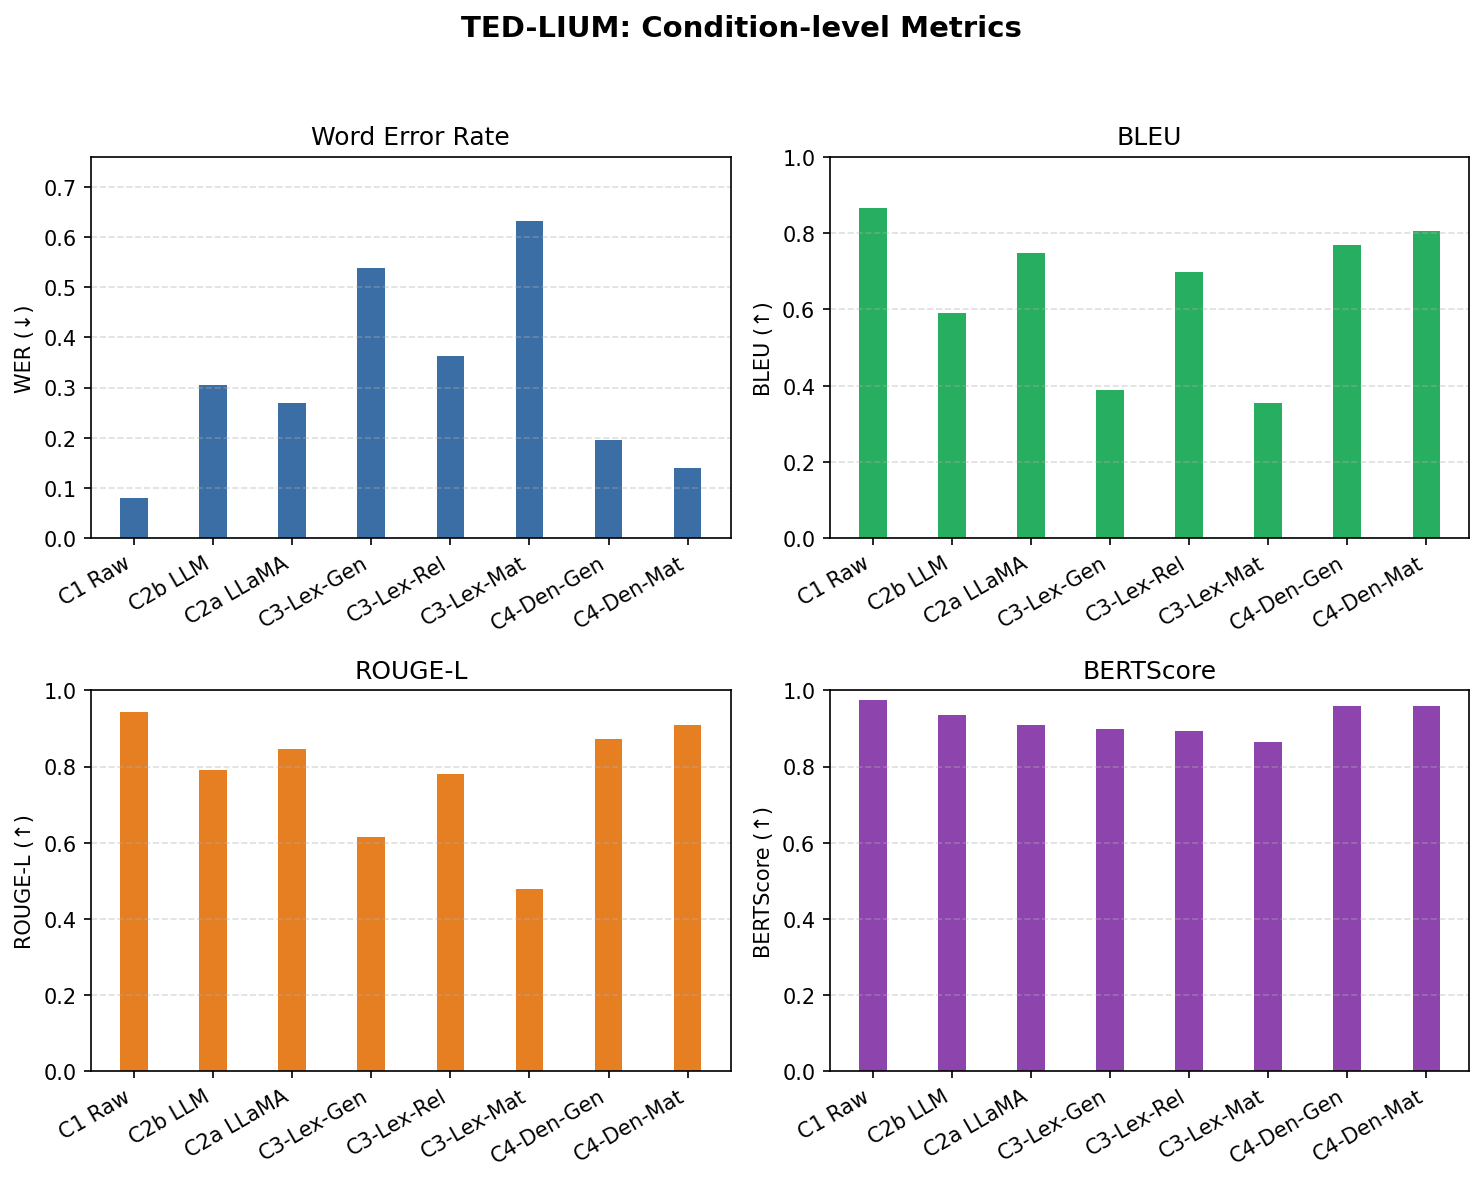
\includegraphics[width=0.96\textwidth]{ted_cond_metrics.png}
  \caption{TED-LIUM condition-level metrics (WER, BLEU, ROUGE-L, BERTScore).
    C4-Den-Mat is best among corrected conditions on all four.
    (Condition labels as in Table~\ref{tab:conditions}.)}
  \label{fig:ted_cond}
\end{figure*}

\begin{figure*}[!htbp]
\centering
  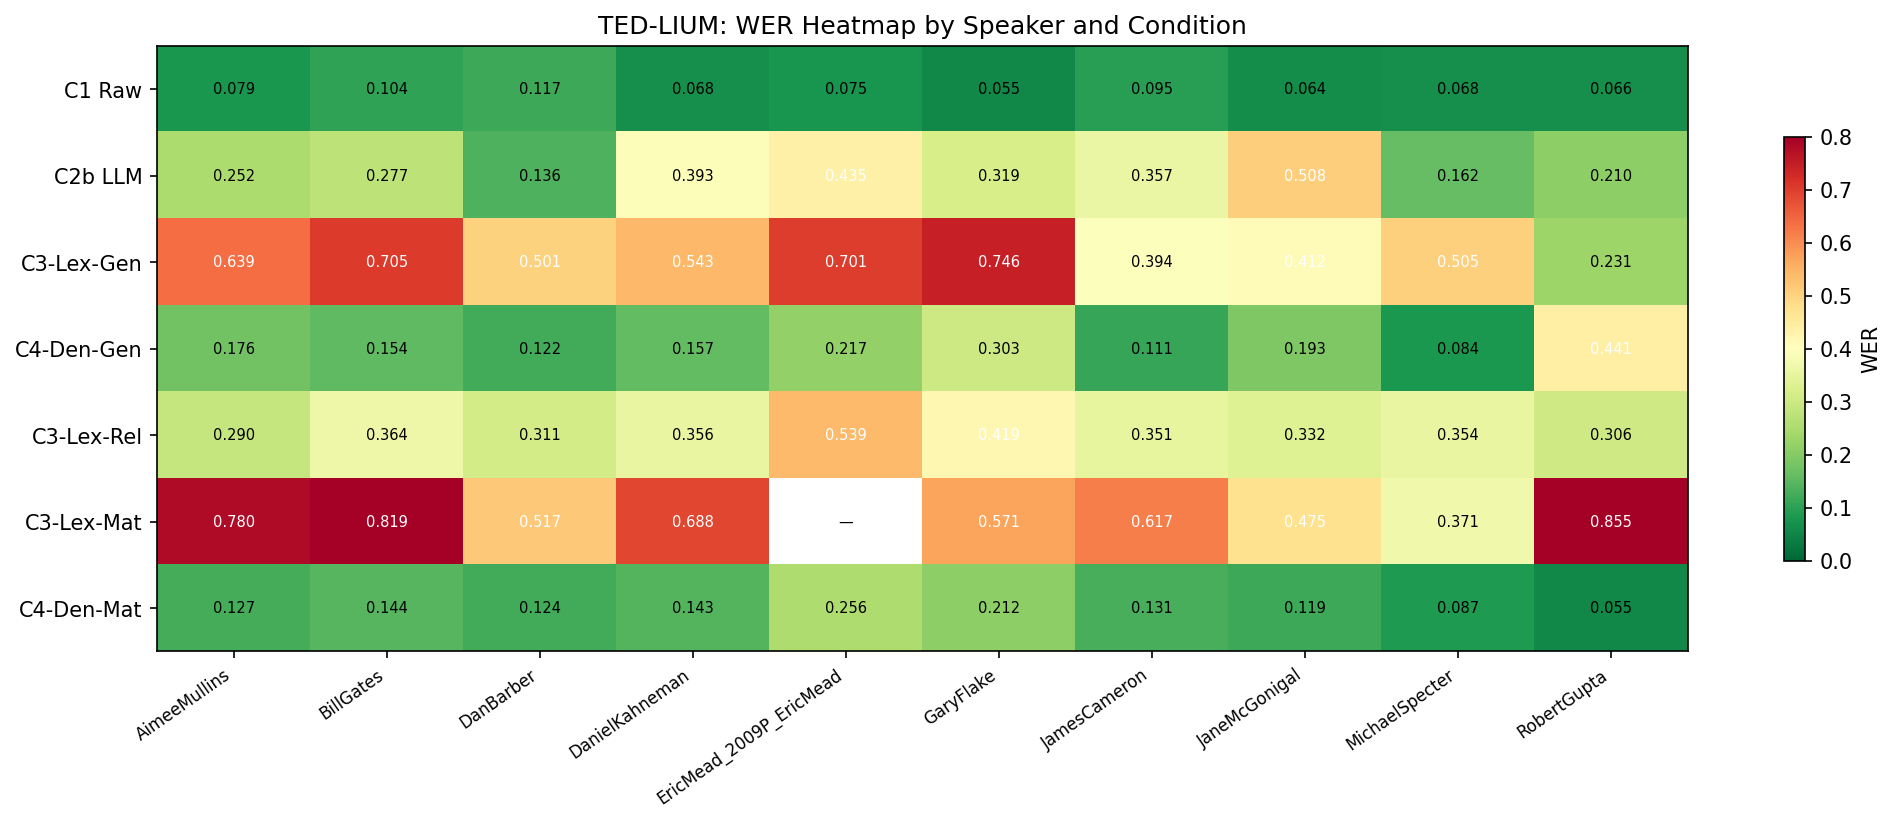
\includegraphics[width=0.96\textwidth]{ted_wer_heat.png}
  \caption{TED-LIUM WER heatmap over 10 speakers and 7 conditions. Blank cell:
    EricMead C3-Lex-Mat excluded (\texttt{"too\_short"}).
    (Condition labels as in Table~\ref{tab:conditions}.)}
  \label{fig:heatmap}
\end{figure*}

\begin{figure*}[!htbp]
  \centering
  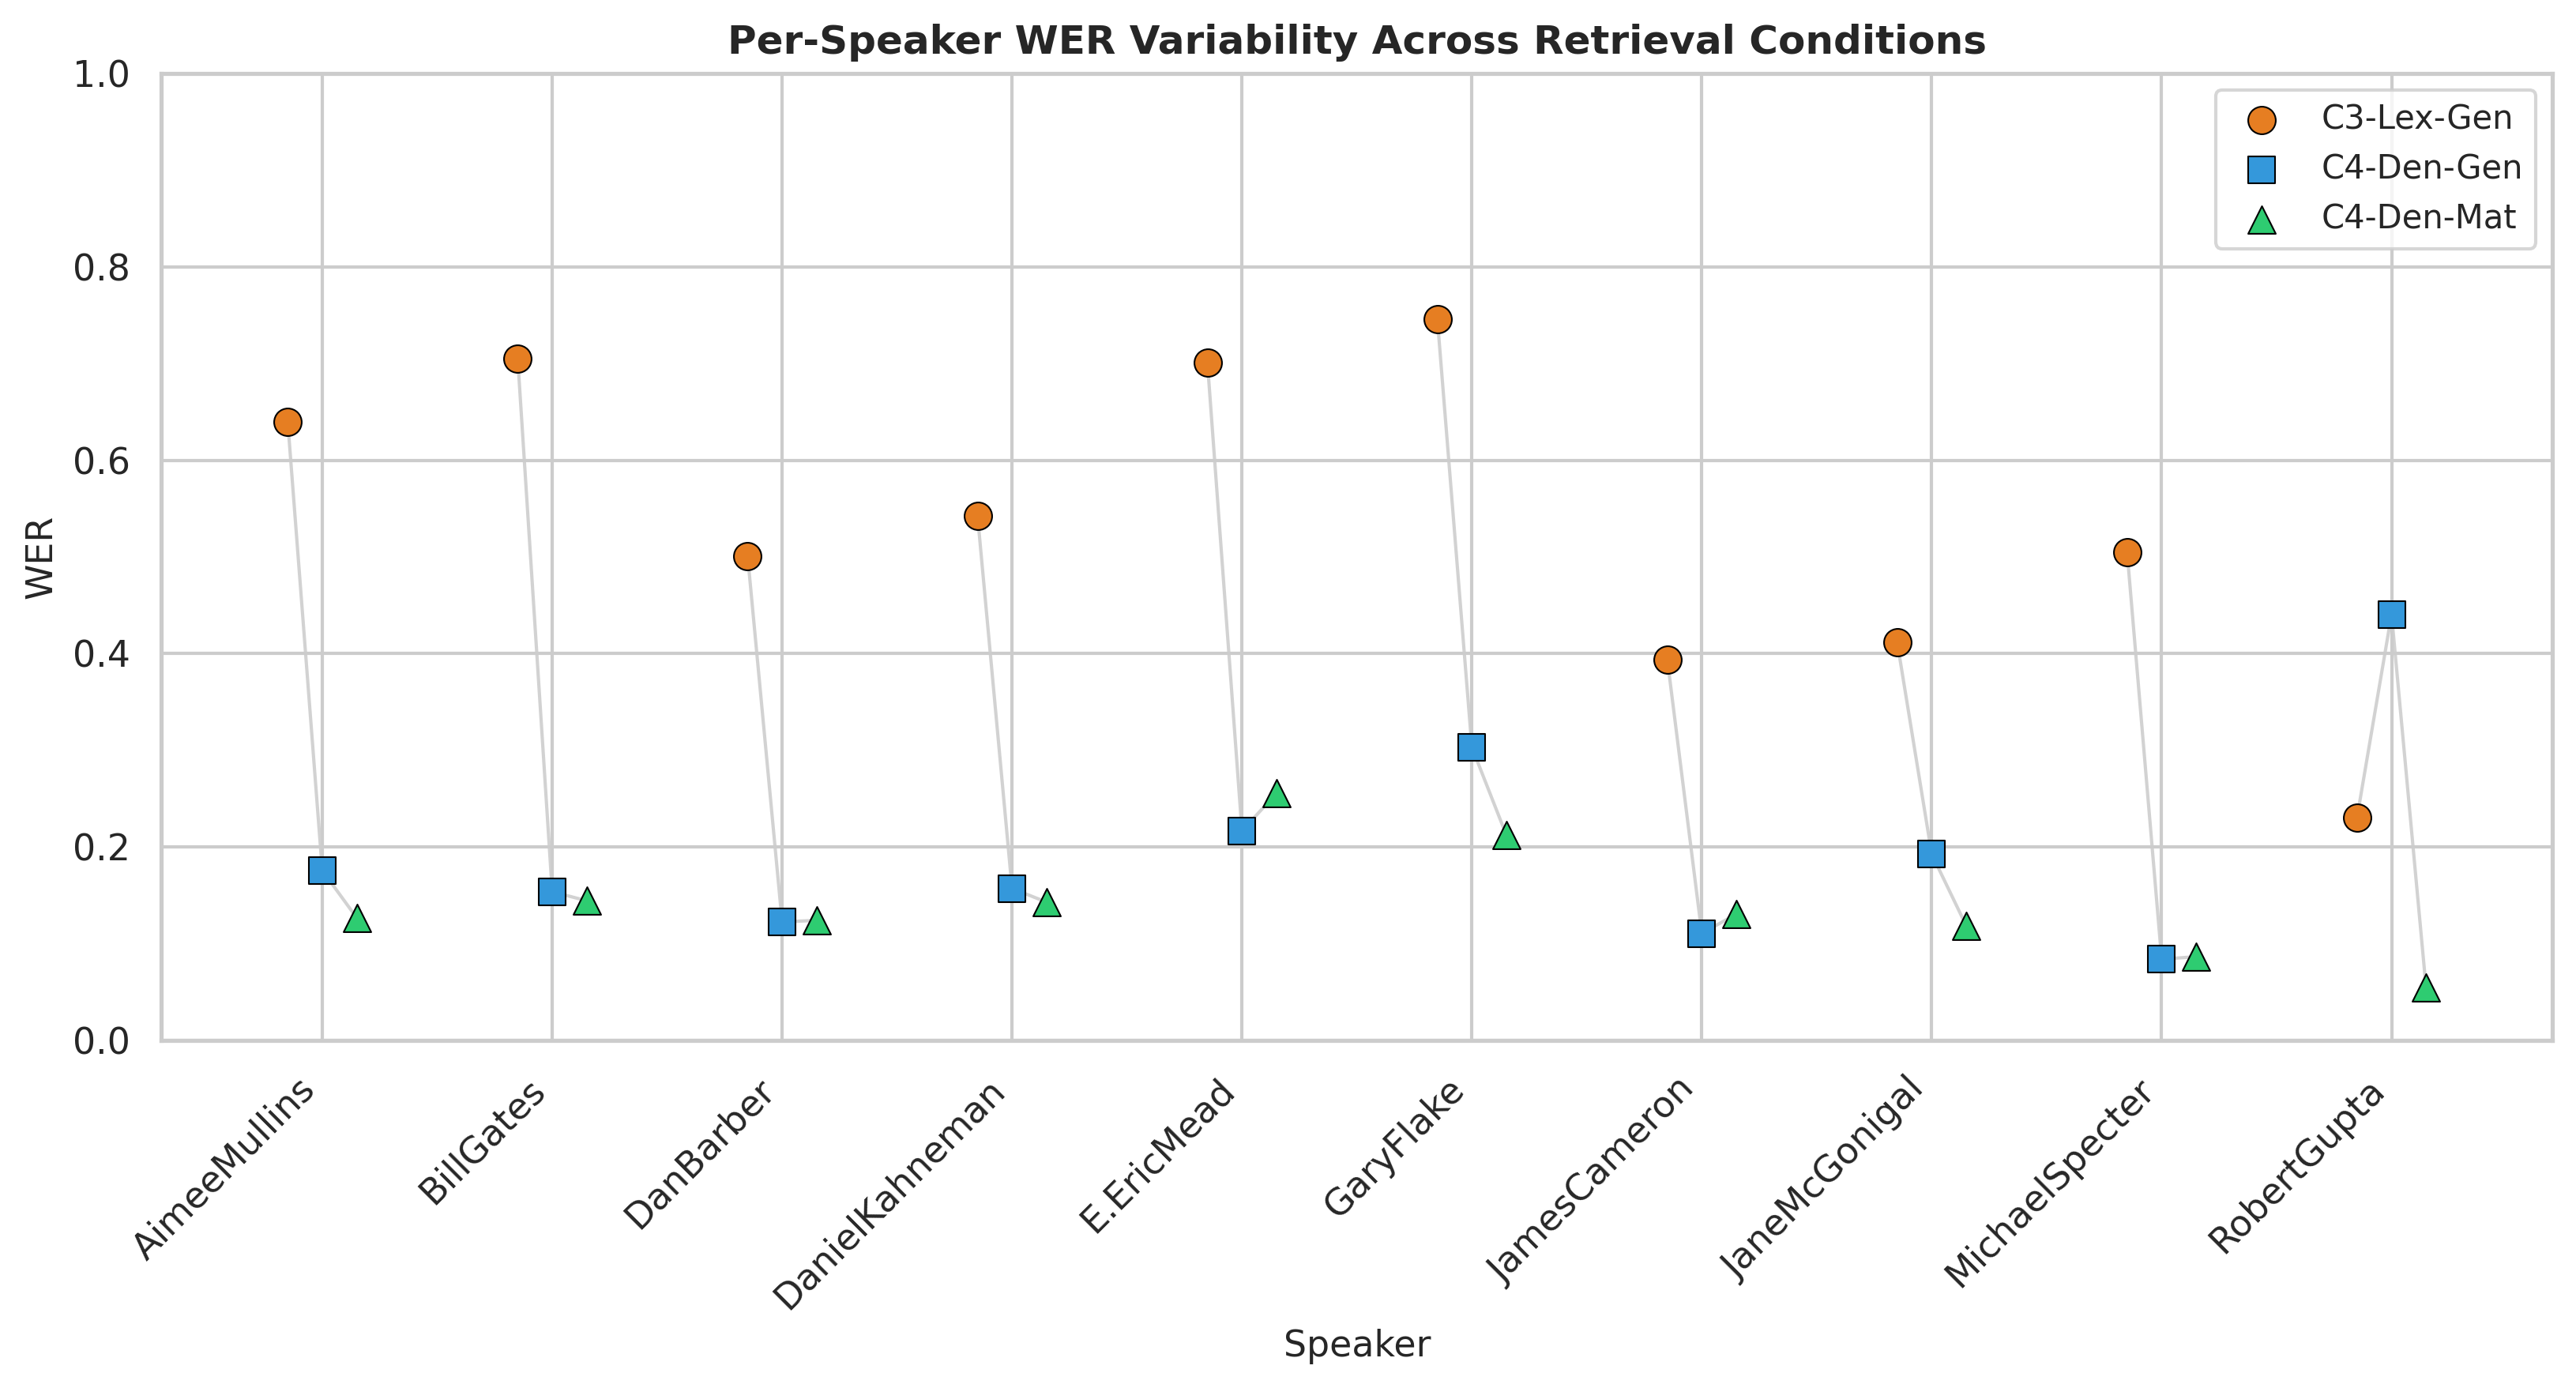
\includegraphics[width=0.96\textwidth]{retrieval_luck.png}
  \caption{Per-speaker WER variance for BM25 generic retrieval (C3-Lex-Gen):
    outcomes follow incidental topical overlap between Wikipedia and each
    speaker's talk, not systematic correction.
    (Condition labels as in Table~\ref{tab:conditions}.)}
  \label{fig:retrieval_luck}
\end{figure*}

\subsection{Statistical Significance (TED-LIUM)}
\label{sec:ted-sig}

Wilcoxon signed-rank tests ($\alpha = 0.05$, $n{=}10$, two-tailed) were used to
compare key condition pairs on TED-LIUM. C4-Den-Mat beats C2b on all four
metrics ($p \leq 0.05$, three at $p{=}0.002$), confirming that dense,
domain-matched retrieval yields consistent gains over an LLM-only baseline on
clean speech. C4-Den-Gen beats C3-Lex-Gen on all metrics ($p{=}0.002$); when
the corpus is fixed, modality alone (dense vs.\ lexical retrieval) strongly
affects performance. Within BM25, C3-Lex-Rel beats C3-Lex-Gen on WER, BLEU, and
ROUGE-L ($p < 0.01$) but not BERTScore ($p{=}0.70$), indicating that better
corpora improve surface overlap more than semantic similarity. C4-Den-Mat vs
C4-Den-Gen is not significant at $n{=}10$, suggesting that both dense
conditions are competitive on clean TED. In contrast, C4-Den-Mat vs
C3-Lex-Mat is significant on all metrics ($p < 0.01$), underlining that when
retrieval is constrained to a strong domain-matched corpus, dense retrieval is
markedly safer than BM25.

\subsection{MTS-Dialog}
\label{sec:mts_results}

Table~\ref{tab:mts} gives aggregate results. C1 has the lowest WER (0.157) and
strong ROUGE-L, reflecting that the synthetic noise process preserves most
reference tokens. Among corrected conditions, LLaMA-only (C2a) is best on all
semantic metrics and NER F1, showing that a well-prompted LLM can clean up
simulated noise without retrieval. Within BM25, domain-relevant and
domain-matched corpora (C3-Lex-Rel/Mat) substantially worsen WER and NER
despite reasonable BLEU/ROUGE-L. Dense retrieval on the same corpora (C4 rows)
shows the same pattern: generic dense (C4-Den-Gen) is relatively safe, while
clinical dense (C4-Den-Mat) produces extreme verbosity and WER 10.25 (marked
$\ddagger$), a first sign of the clinical corpus penalty.

Table~\ref{tab:ner-by-type} and Figure~\ref{fig:mts_metrics} make this penalty
visible at the entity level. CHEMICAL and DISEASE F1 peak for C2a and remain
high for C4-Den-Gen, but drop sharply for the clinical corpora (C3-Lex-Rel/Mat,
C4-Den-Rel/Mat): the model follows plausible but wrong entity strings from
retrieved MTS-Dialog passages even when surface metrics look acceptable. The
Wilcoxon tests in Table~\ref{tab:mts_wilcoxon} confirm that these differences
are statistically reliable at $n{=}100$.

\begin{table*}[!t]
\centering
\caption{Average results on MTS-Dialog (100 dialogues). $\ddagger$ = WER
inflated by verbosity. \best\ = best corrected. NER: spaCy
\texttt{en\_core\_web\_sm}; CHEM/DIS: scispaCy \texttt{en\_ner\_bc5cdr\_md}.}
\label{tab:mts}
\footnotesize
\setlength{\tabcolsep}{3.5pt}
\renewcommand{\arraystretch}{1.1}
\begin{tabular}{lccccccc}
\toprule
\textbf{Condition} & \textbf{WER\,\dn} & \textbf{BLEU\,\up} & \textbf{RG-L\,\up} & \textbf{BERT\,\up} & \textbf{NER\,\up} & \textbf{CHEM\,\up} & \textbf{DIS\,\up} \\
\midrule
C1 Baseline     & \bestnum{0.157} & 0.694 & \bestnum{0.912} & 0.959 & \bestnum{0.766} & 0.918 & 0.922 \\
\midrule
C2b LLM-Only    & 0.241 & 0.658 & 0.852 & 0.962 & 0.650 & 0.933 & 0.935 \\
C2a LLaMA~\best & \bestnum{0.207} & \bestnum{0.717} & \bestnum{0.877} & \bestnum{0.963} & \bestnum{0.740} & \bestnum{0.938} & \bestnum{0.937} \\
\midrule
\multicolumn{8}{l}{\small\textit{BM25 Lexical}} \\
C3-Lex-Gen      & 0.265  & 0.621 & 0.822 & 0.956 & 0.669 & 0.945 & 0.926 \\
C3-Lex-Rel      & 0.917  & 0.537 & 0.737 & 0.941 & 0.563 & 0.848 & 0.822 \\
C3-Lex-Mat      & 1.028  & 0.472 & 0.665 & 0.926 & 0.505 & 0.851 & 0.744 \\
\midrule
\multicolumn{8}{l}{\small\textit{Dense Embedding}} \\
C4-Den-Gen      & 0.237  & 0.645 & 0.838 & 0.961 & 0.681 & 0.935 & 0.913 \\
C4-Den-Rel      & 1.024  & 0.500 & 0.707 & 0.934 & 0.506 & 0.827 & 0.834 \\
C4-Den-Mat$^\ddagger$ & 10.25 & 0.513 & 0.726 & 0.943 & 0.543 & 0.890 & 0.837 \\
\bottomrule
\end{tabular}
\end{table*}

\begin{table}[t]
\centering
\caption{NER F1 by entity type on MTS-Dialog (100 dialogues).
  General: spaCy \texttt{en\_core\_web\_sm};
  Biomedical: scispaCy \texttt{en\_ner\_bc5cdr\_md}.}
\label{tab:ner-by-type}
\footnotesize
\setlength{\tabcolsep}{3.5pt}
\renewcommand{\arraystretch}{1.05}
\begin{tabular}{lrrr}
\toprule
Condition & General NER & CHEMICAL & DISEASE \\
\midrule
C1 Baseline     & 0.766 & 0.918 & 0.922 \\
C2b LLM-Only    & 0.650 & 0.933 & 0.935 \\
C2a LLaMA       & 0.740 & 0.938 & 0.937 \\
C3-Lex-Gen      & 0.669 & 0.945 & 0.926 \\
C3-Lex-Rel      & 0.563 & 0.848 & 0.822 \\
C3-Lex-Mat      & 0.505 & 0.851 & 0.744 \\
C4-Den-Gen      & 0.681 & 0.935 & 0.913 \\
C4-Den-Rel      & 0.506 & 0.827 & 0.834 \\
C4-Den-Mat      & 0.543 & 0.890 & 0.837 \\
\bottomrule
\end{tabular}
\end{table}

\begin{figure*}[!htbp]
  \centering
  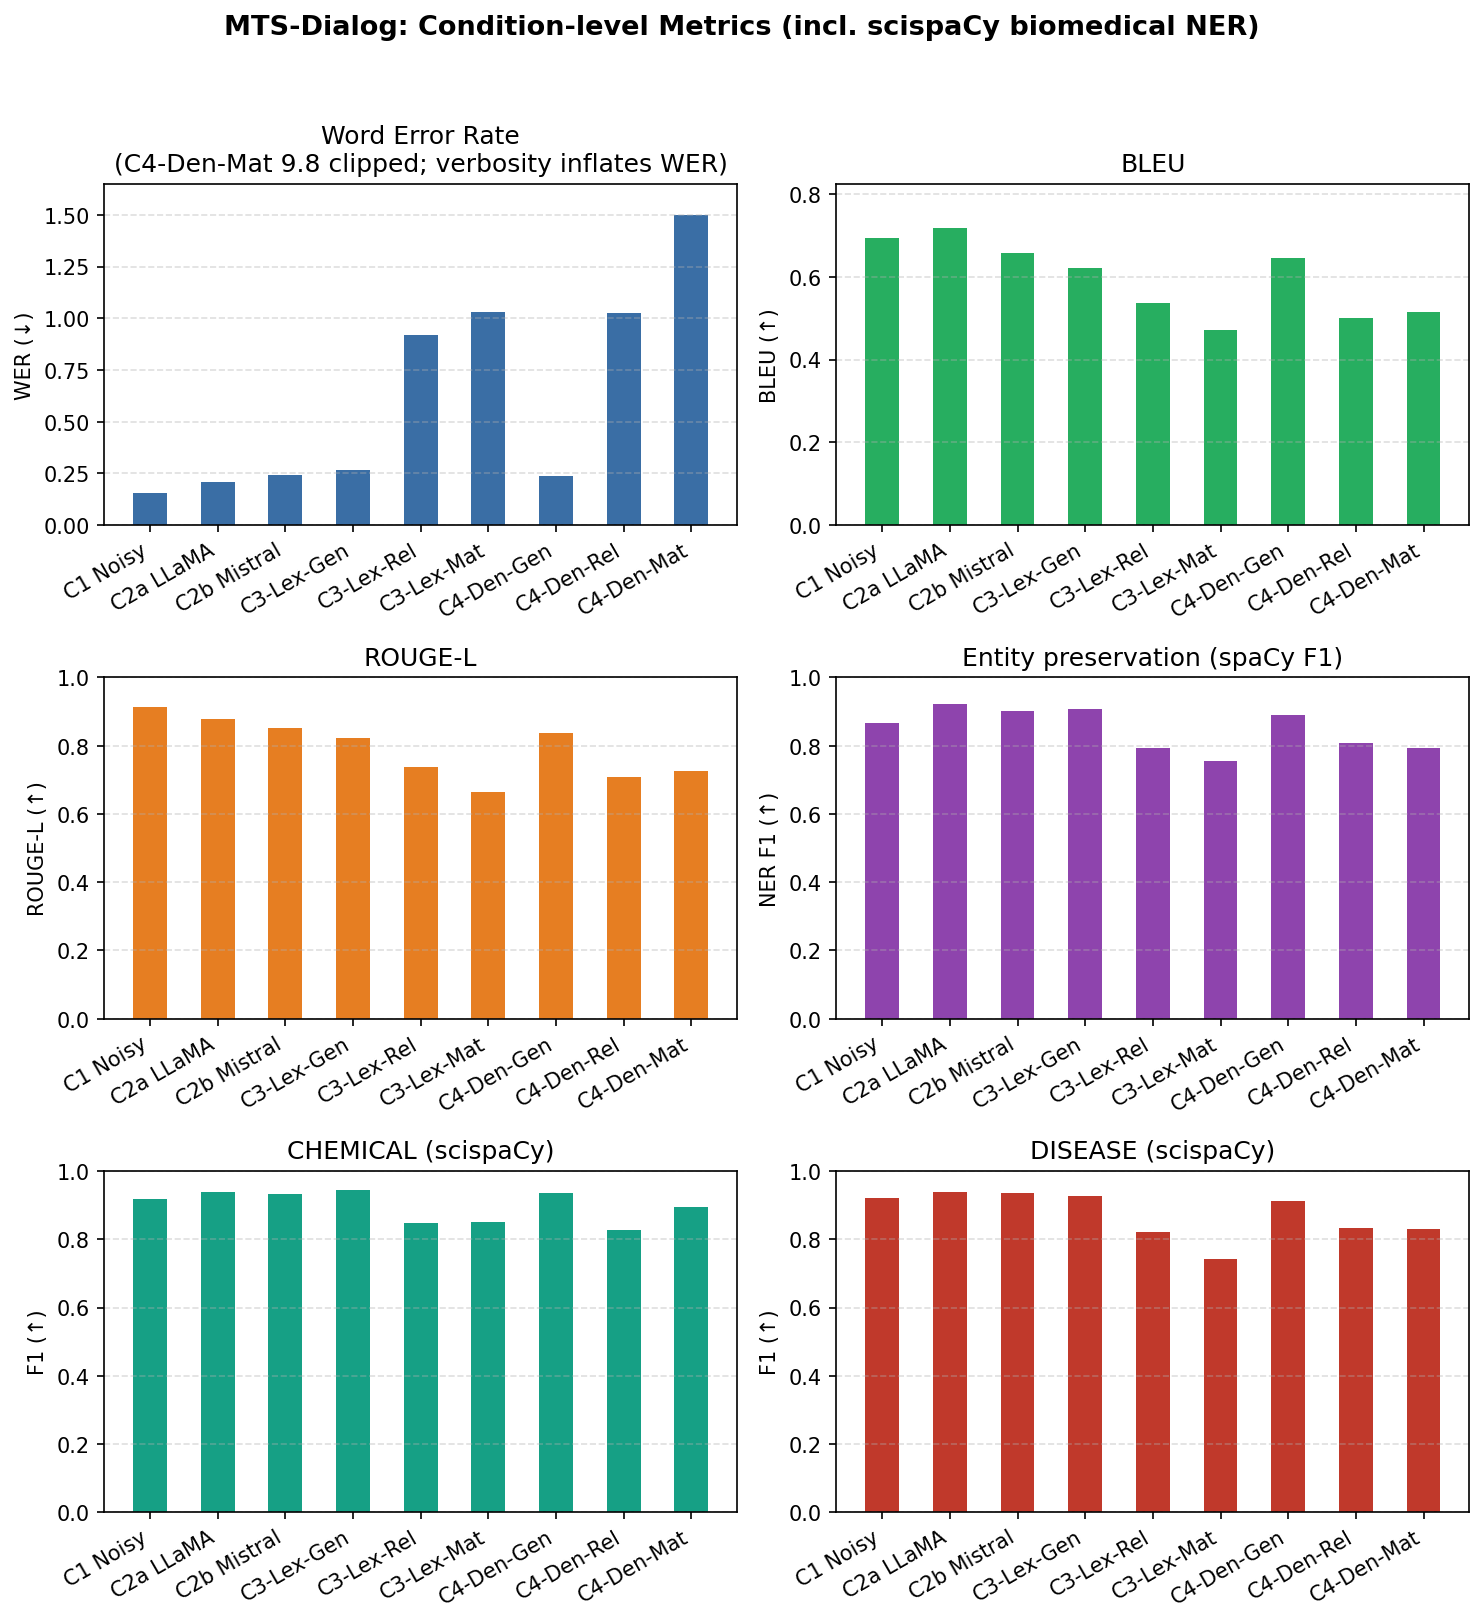
\includegraphics[width=0.96\textwidth]{mts_cond_metrics.png}
  \caption{MTS-Dialog condition-level metrics including biomedical NER
    (scispaCy). LLaMA-Only (C2a) has the highest NER F1 among corrected
    conditions. (Condition labels as in Table~\ref{tab:conditions}.)}
  \label{fig:mts_metrics}
\end{figure*}

\subsection{Statistical Significance (MTS-Dialog)}
\label{sec:mts_sig}

Paired Wilcoxon signed-rank tests (two-tailed, $\alpha = 0.05$, $n{=}100$) are
in Table~\ref{tab:mts_wilcoxon}. Per-dialogue metrics were saved for all 100
dialogues.

\begin{table}[!t]
\centering
\caption{Wilcoxon results (MTS-Dialog, $n{=}100$). $^\ast$ = scispaCy
\texttt{en\_ner\_bc5cdr\_md}.}
\label{tab:mts_wilcoxon}
\footnotesize
\setlength{\tabcolsep}{3.5pt}
\renewcommand{\arraystretch}{1.1}
\begin{tabular}{p{2.4cm}lcc}
\toprule
\textbf{Comparison} & \textbf{Metric} & \textbf{\textit{p}} & \textbf{Sig.} \\
\midrule
\multirow{6}{*}{C4-Den-Mat vs C2b}
  & WER                     & \cellcolor{siggreen}$<$0.01  & Yes \\
  & BLEU                    & \cellcolor{siggreen}$<$0.01  & Yes \\
  & ROUGE-L                 & \cellcolor{siggreen}$<$0.01  & Yes \\
  & BERTScore               & \cellcolor{siggreen}$<$0.01  & Yes \\
  & CHEMICAL F1$^\ast$      & \cellcolor{sigunsig}0.141    & No  \\
  & DISEASE F1$^\ast$       & \cellcolor{siggreen}0.0013   & Yes \\
\midrule
\multirow{2}{*}{\parbox{2.4cm}{C4-Den-Mat vs\\C4-Den-Gen}}
  & DISEASE F1$^\ast$       & \cellcolor{siggreen}0.0098   & Yes \\
  & scispaCy overall$^\ast$ & \cellcolor{siggreen}0.0056   & Yes \\
\midrule
\multirow{4}{*}{\parbox{2.4cm}{C4-Den-Mat vs\\C4-Den-Rel}}
  & WER       & \cellcolor{sigunsig}$>$0.05 & No \\
  & BLEU      & \cellcolor{sigunsig}$>$0.05 & No \\
  & ROUGE-L   & \cellcolor{sigunsig}$>$0.05 & No \\
  & BERTScore & \cellcolor{sigunsig}$>$0.05 & No \\
\midrule
\multirow{4}{*}{\parbox{2.4cm}{C4-Den-Rel vs\\C3-Lex-Rel}}
  & WER       & \cellcolor{sigunsig}0.071  & No  \\
  & BLEU      & \cellcolor{siggreen}0.029  & Yes \\
  & ROUGE-L   & \cellcolor{siggreen}0.039  & Yes \\
  & BERTScore & \cellcolor{siggreen}0.043  & Yes \\
\midrule
\multirow{4}{*}{C2a vs C2b}
  & WER       & \cellcolor{sigunsig}$>$0.05 & No  \\
  & BLEU      & \cellcolor{siggreen}$<$0.01 & Yes \\
  & ROUGE-L   & \cellcolor{sigunsig}$>$0.05 & No  \\
  & BERTScore & \cellcolor{sigunsig}$>$0.05 & No  \\
\bottomrule
\end{tabular}
\end{table}

\subsection{PriMock57 (Real Clinical Audio)}
\label{sec:primock57_results}

Table~\ref{tab:primock57} gives mean WER over ten consultations.
C4-Den-Mat on PriMock57 uses leave-one-out PriMock57 (domain-matched), as does
C3-Lex-Mat.
The full metric set (WER, BLEU, ROUGE-L, BERTScore, CHEMICAL F1, DISEASE F1)
for all seven corrected conditions is shown in Figure~\ref{fig:primock57_metrics}.

\begin{table}[!t]
\centering
\caption{Mean WER on PriMock57 ($n{=}10$). \best\ = best condition.}
\label{tab:primock57}
\footnotesize
\setlength{\tabcolsep}{3.5pt}
\renewcommand{\arraystretch}{1.05}
\begin{tabular}{lcp{3.2cm}}
\toprule
\textbf{Condition} & \textbf{WER\,\dn} & \textbf{Notes} \\
\midrule
C1 (Whisper)      & 0.872 & ASR baseline \\
\midrule
C2b (Mistral)~\best & \bestnum{0.869} & LLM-only; best overall \\
C2a (LLaMA)       & 0.925 & \\
\midrule
\multicolumn{3}{l}{\small\textit{BM25 Lexical}} \\
C3-Lex-Gen        & 0.960 & \\
C3-Lex-Rel        & 1.033 & \\
C3-Lex-Mat        & 0.997 & \\
\midrule
\multicolumn{3}{l}{\small\textit{Dense Embedding}} \\
C4-Den-Gen        & 0.902 & Best RAG condition \\
C4-Den-Mat        & 0.991 & Leave-one-out PriMock57 (domain-matched) \\
\bottomrule
\end{tabular}
\end{table}

No condition clearly beats the 0.872 baseline. C2b (WER 0.869) is slightly
best, with C1 and C4-Den-Gen close behind. C4-Den-Mat (WER 0.991) is 14\%
worse than C2b in relative terms, and the clinical lexical conditions
(C3-Lex-Rel/Mat) are also worse than LLM-only. C1 leads on BLEU, ROUGE-L,
and NER because Whisper keeps many reference surface forms; LLM and RAG
outputs paraphrase and substitute formal terminology, which exact-match
metrics penalise even when meaning is preserved. Figure~\ref{fig:primock57_metrics}
shows that these patterns hold across CHEMICAL and DISEASE F1 as well: generic
or LLM-only correction is safer than consultation-non-specific clinical
retrieval.

\subsection{Extended Evaluation: PriMock57 Full 57 Consultations}
\label{sec:primock57_full}

\begin{table}[!t]
\centering
\caption{Mean metrics, PriMock57 full ($n{=}57$).}
\label{tab:primock57_57}
\footnotesize
\setlength{\tabcolsep}{3pt}
\renewcommand{\arraystretch}{1.05}
\begin{tabular}{lcccc}
\toprule
\textbf{Condition} & \textbf{WER\,\dn} & \textbf{BLEU\,\up} & \textbf{RG-L\,\up} & \textbf{BERT\,\up} \\
\midrule
C1 (Whisper)  & 0.821        & \bestnum{0.495} & \bestnum{0.498} & 0.838 \\
C2b (Mistral) & \bestnum{0.820} & 0.036        & 0.296        & \bestnum{0.840} \\
C4-Den-Mat    & 0.881        & 0.024        & 0.201        & 0.826 \\
\bottomrule
\end{tabular}
\end{table}

\begin{table}[!t]
\centering
\caption{Wilcoxon results, C4-Den-Mat vs C2b, PriMock57 full ($n{=}57$).}
\label{tab:primock57_wilcoxon}
\footnotesize
\setlength{\tabcolsep}{3.5pt}
\renewcommand{\arraystretch}{1.05}
\begin{tabular}{lcc}
\toprule
\textbf{Metric} & \textbf{\textit{p}-value} & \textbf{Sig.} \\
\midrule
WER       & \cellcolor{siggreen}$<$0.001 & Yes \\
BLEU      & \cellcolor{siggreen}0.004    & Yes \\
ROUGE-L   & \cellcolor{siggreen}$<$0.001 & Yes \\
BERTScore & \cellcolor{siggreen}$<$0.001 & Yes \\
\bottomrule
\end{tabular}
\end{table}

C4-Den-Mat is worse than C2b on all four metrics ($p < 0.01$). C2b and C1 are
not distinguishable at the WER level, confirming that dense clinical retrieval
introduces a systematic degradation relative to a plain LLM-only correction
step. The magnitude of the WER gap (0.881 vs 0.820) is modest in absolute
terms but statistically robust, and is accompanied by consistent drops in
BLEU, ROUGE-L, and BERTScore. Taken together with the ten-consultation pilot,
the full 57-consultation run shows that, under the current ASR quality and
retrieval setup, clinical dense RAG does not recover phonetic errors from text
context and instead tends to add clinically plausible but locally incorrect
material.

\vspace{-2pt}
\FloatBarrier
\subsection{Hypothesis Summary}
\label{sec:hypotheses}

\begin{itemize}[leftmargin=1.2em, itemsep=0pt, topsep=0pt, parsep=0pt, partopsep=0pt]
  \item \textbf{H1 (RAG vs.\ LLM-only):} supported on TED; C4-Den-Gen and
    C4-Den-Mat beat C2b, while C3-Lex-Gen is worse (retrieval quality matters).
  \item \textbf{H2 (domain-specific vs.\ generic):} supported on TED; C4-Den-Mat
    is best (WER 0.140, ROUGE-L 0.905).
  \item \textbf{H3 (dense vs.\ lexical):} supported on TED (62\% WER reduction,
    $p < 0.01$); on MTS, WER is not significant ($p = 0.071$) but BLEU/ROUGE-L/
    BERTScore are ($p < 0.05$).
  \item \textbf{H4 (RAG on noisy clinical):} not supported on PriMock57. C4-Den-Mat
    is significantly worse than C2b on all four metrics (WER, BLEU, ROUGE-L,
    BERTScore; $p < 0.01$) and degrades DISEASE F1; generic retrieval is safer
    for biomedical entities.
\end{itemize}

\begin{figure*}[!htbp]
  \centering
  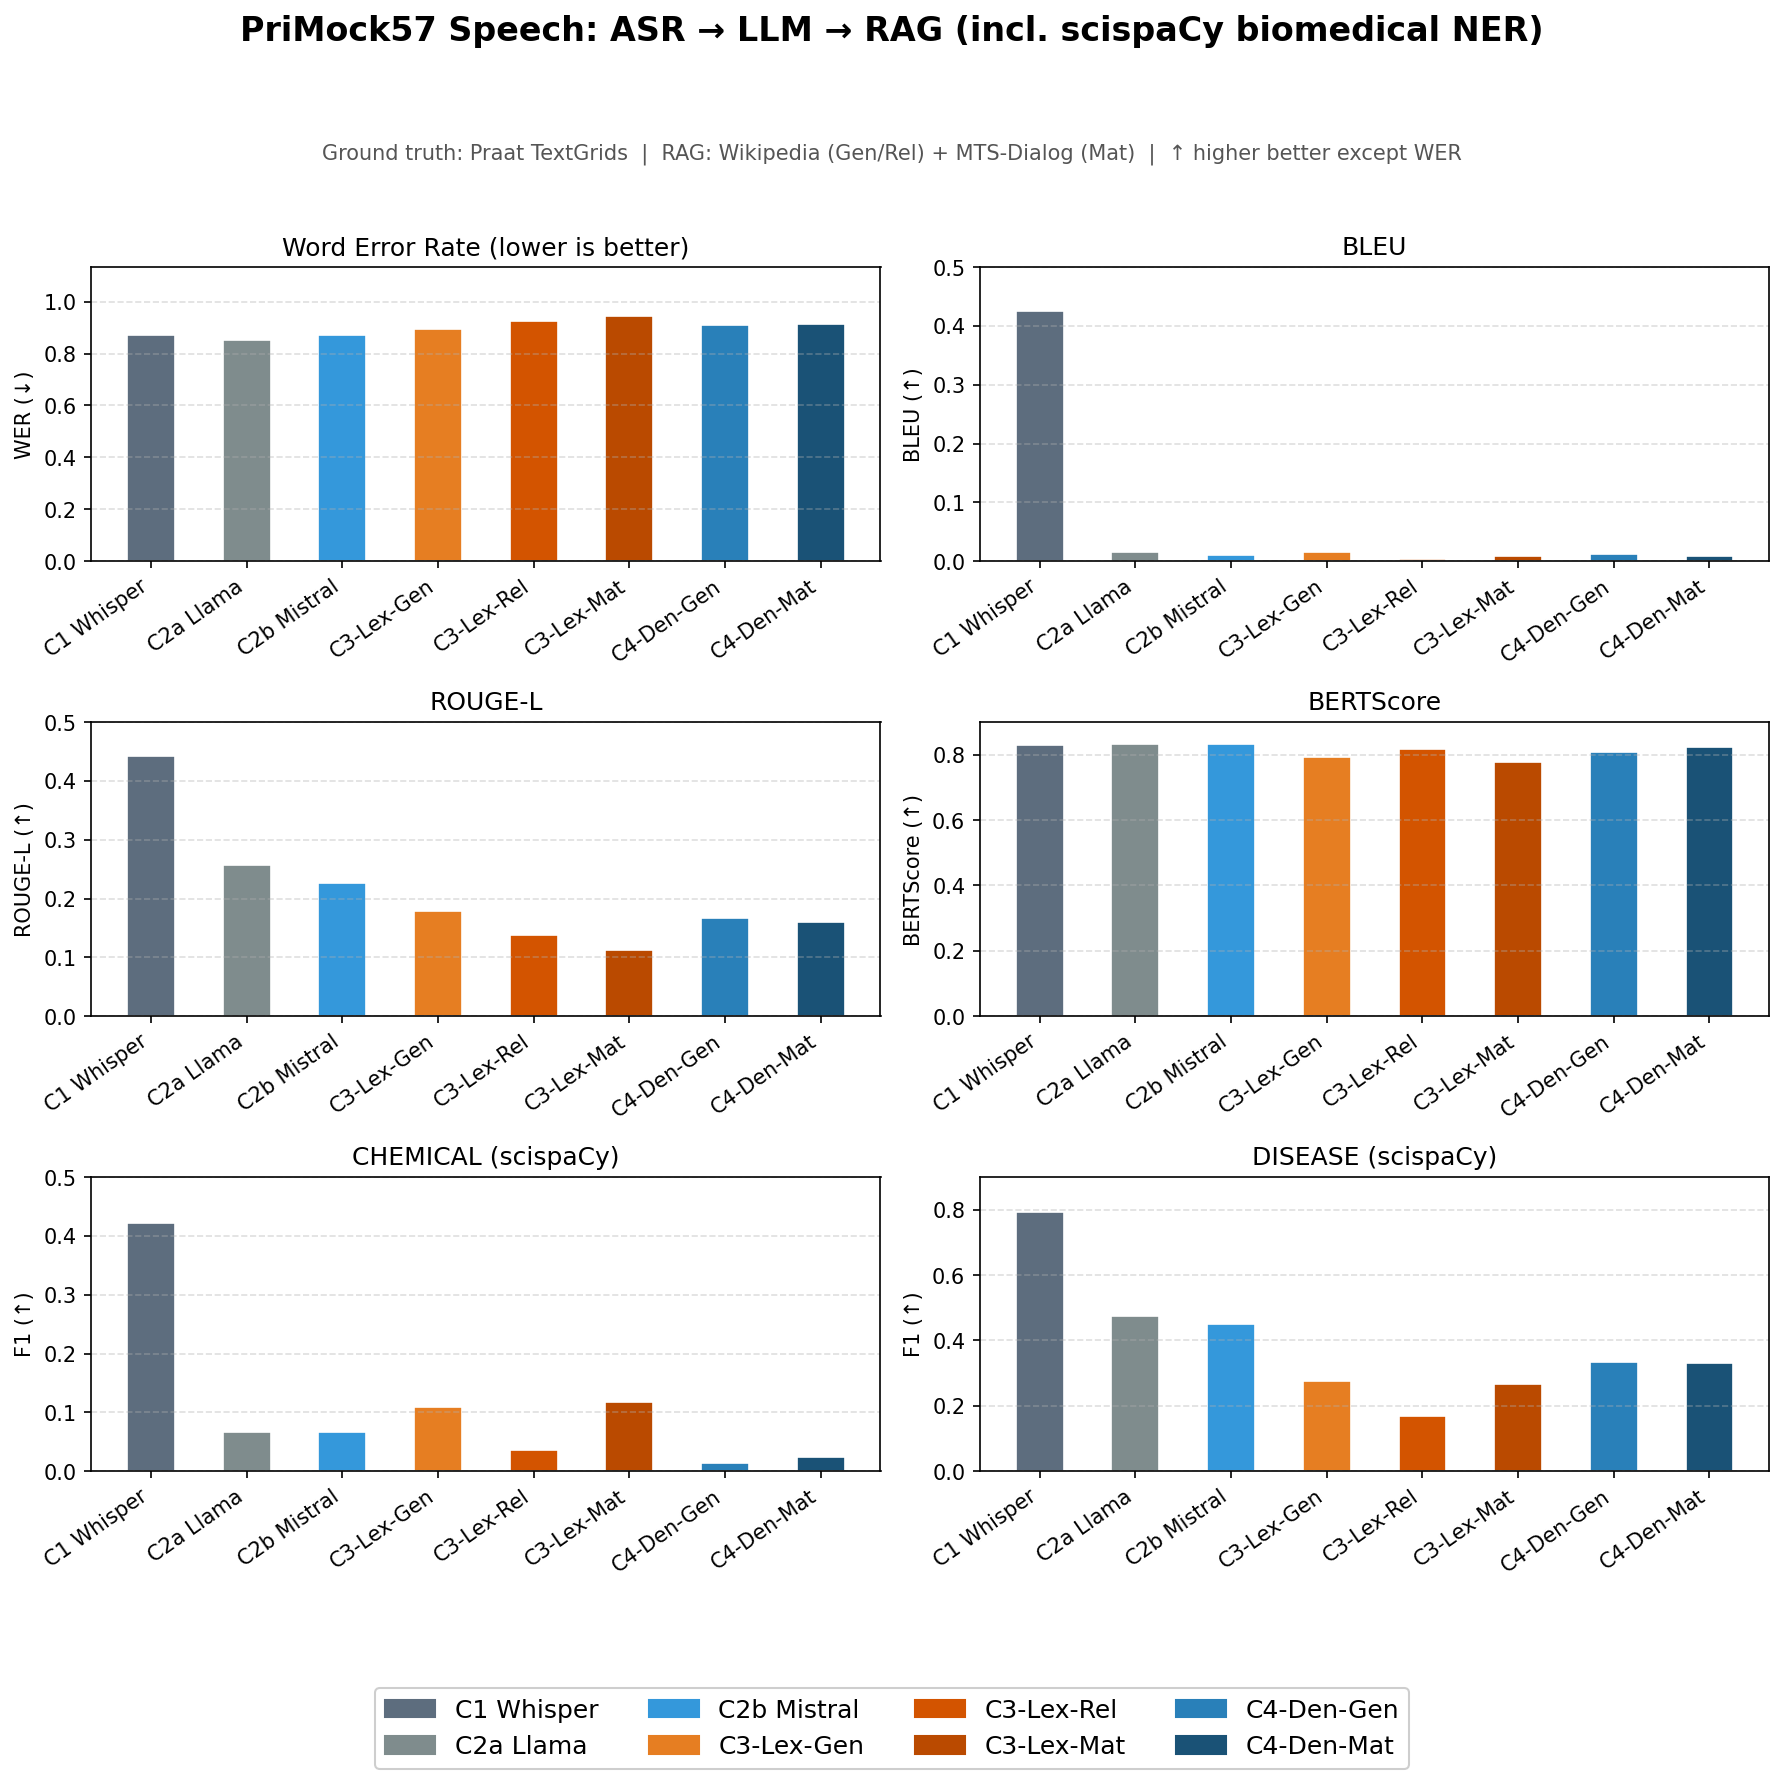
\includegraphics[width=\textwidth]{primock57_speech_cond_metrics.png}
  \caption{PriMock57: WER, BLEU, ROUGE-L, BERTScore, CHEMICAL F1, DISEASE F1
    over seven corrected conditions ($n{=}10$). C1 leads on BLEU, ROUGE-L, NER;
    C2b is numerically best on WER and BERTScore (C2b and C1 are not statistically
    distinguished on WER); C4-Den-Mat is worse than C2b on all four text metrics. (Condition labels as in Table~\ref{tab:conditions}.)}
  \label{fig:primock57_metrics}
\end{figure*}

\FloatBarrier
\section{Discussion}

\subsection{Retrieval Corpus and Modality Effects}

Results show a strong interaction between retrieval modality and corpus scope.
On TED-LIUM, generic lexical retrieval (C3-Lex-Gen) substantially worsens
performance (WER 0.516), whereas dense retrieval on the same corpus
(C4-Den-Gen) reduces WER by 62\% ($p < 0.01$). Within BM25, corpus
matters (C3-Lex-Rel 0.362 vs C3-Lex-Gen; BERTScore $p = 0.70$). Domain
alignment amplifies gains: C4-Den-Mat 54\% WER reduction over C2b, C4-Den-Gen
36\%. PriMock57 C4-Den-Mat uses leave-one-out PriMock57 (domain-matched), same
corpus as C3-Lex-Mat.

These patterns reflect different underlying acoustic regimes. On TED-LIUM,
Whisper-tiny already achieves WER 0.079 under near-ideal conditions (clean,
single-speaker, rehearsed speech). Any post-correction step that changes tokens
risks mismatching the reference and inflating WER even when meaning is
preserved. Dense RAG can afford mild paraphrase here, as shown by BERTScore
remaining above 0.93 across corrected conditions, whereas BM25 lexical
retrieval tends to inject irrelevant surface forms.

PriMock57 shows the opposite: baseline WER 0.872 leaves ample headroom, but
neither lexical nor dense RAG clearly improves on Mistral-only. The 14\%
relative WER degradation of C4-Den-Mat vs C2b indicates that consultation-
non-specific clinical passages can actively hurt performance when phonetic
errors dominate and the model cannot rely on acoustic cues.

\begin{figure*}[!htbp]
  \centering
  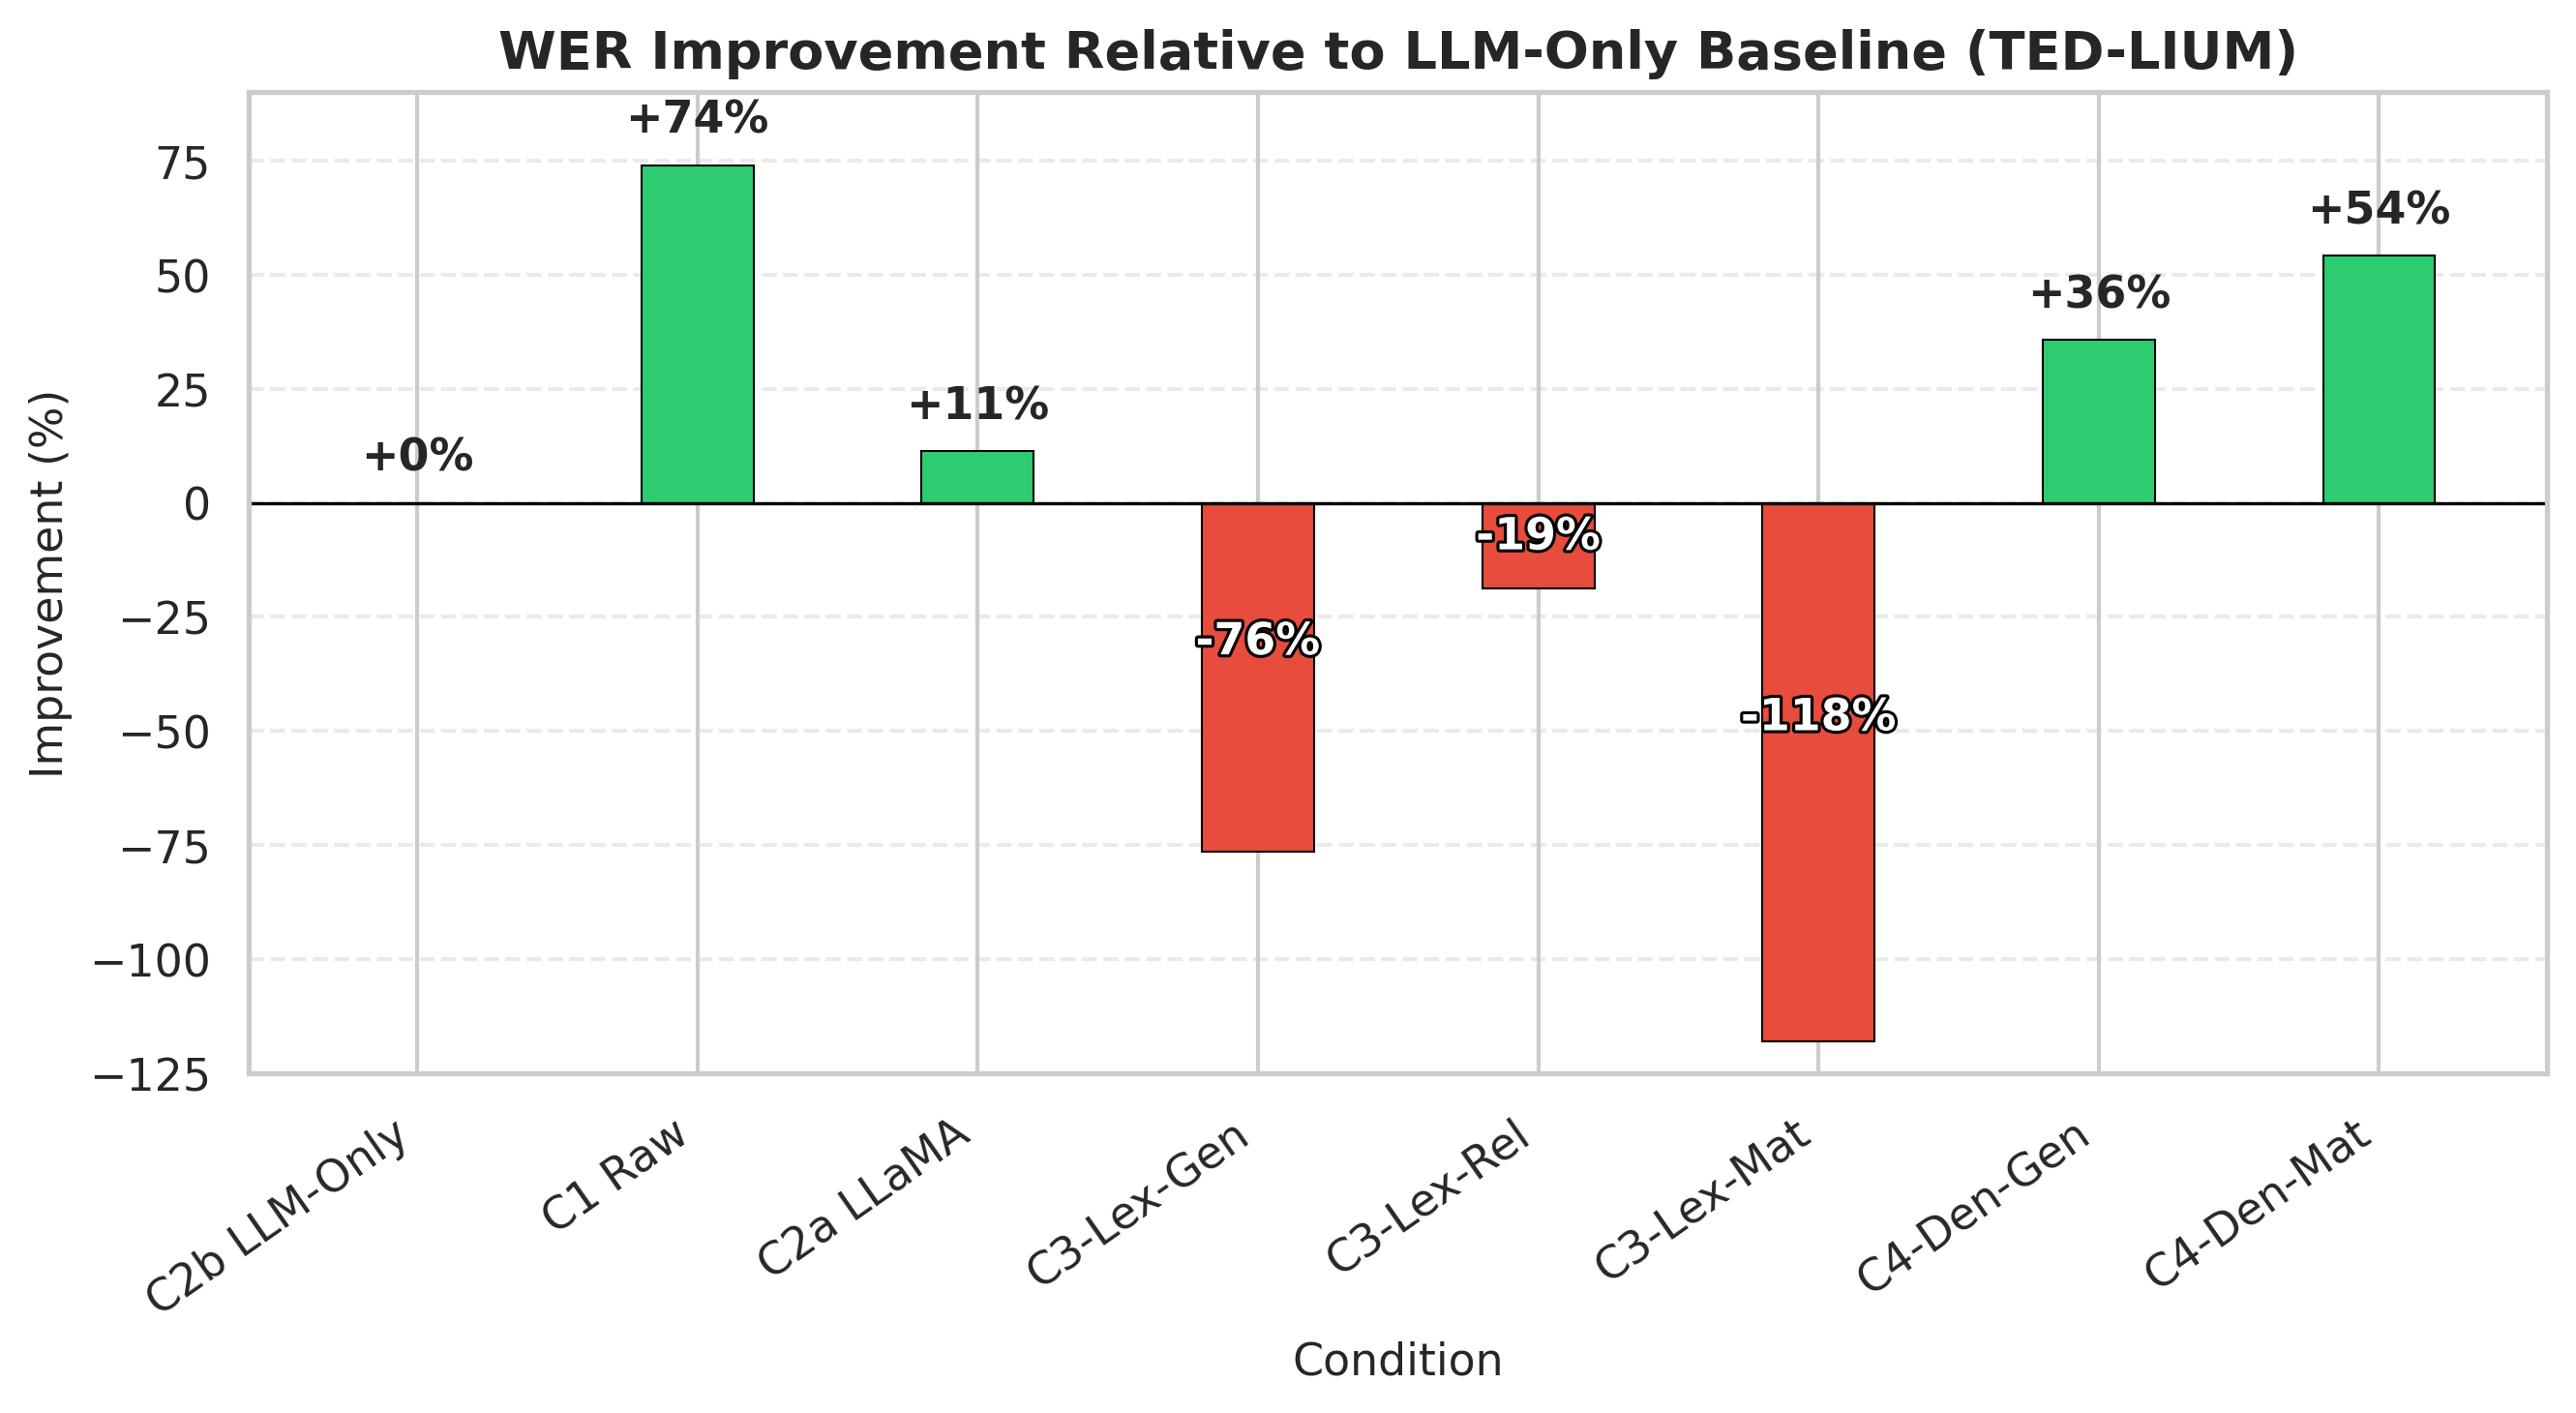
\includegraphics[width=0.98\textwidth]{improvement_chart.png}
  \caption{WER change relative to LLM-Only (TED-LIUM). Positive = WER
    reduction; negative = degradation.}
  \label{fig:wer_improvement}
\end{figure*}

\subsection{Entity Preservation in Clinical Dialogues}
\label{sec:entity}\label{sec:verbosity}

BERTScore and WER diverge in clinical conditions; NER explains why. The
clinical-corpus penalty arises because dense retrieval returns semantically
related clinical passages containing plausible medical entities; when the LLM
encounters uncertain ASR tokens it often substitutes those entities into the
transcript, preserving embedding-based similarity while degrading entity-level
fidelity. General spaCy drops with Mistral (0.650--0.681 vs 0.766);
LLaMA-Only (0.740) highest. ScispaCy: LLM and generic dense (C4-Den-Gen)
preserve or improve DISEASE F1; with clinical corpora, C4-Den-Mat
(DIS 0.837) is worse than C4-Den-Gen ($p = 0.0098$). Plausible-but-wrong
entity substitutions from retrieved passages are invisible to BERTScore
(0.93--0.96) but visible in DISEASE F1 (0.744--0.937);
Table~\ref{tab:ner-by-type} breaks down by type.

The clinical corpus penalty arises from the interaction between dense
retrieval and generative reformulation. Dense retrievers return
semantically related clinical passages containing medically plausible
entities. When the language model encounters uncertain tokens in the ASR
transcript, it often replaces them with entity strings from the retrieved
context. These substitutions maintain high semantic similarity but can
introduce clinically incorrect entities. Because embedding-based metrics
such as BERTScore reward semantic similarity, they remain largely invisible
to standard evaluation metrics but are detected by biomedical NER.

Some C4-Den-Mat outputs had multiple \texttt{TRANSCRIPT} blocks (verbosity; WER
$>$ 1.0), likely prompt-following failure.

The PriMock57 NER behaviour illustrates a subtle evaluation issue. Raw Whisper
often preserves surface forms from the reference transcription, so C1 can lead
on BLEU, ROUGE-L, and NER F1 even when its clinical interpretations are no
better than corrected outputs. LLM and RAG conditions frequently substitute
formal terminology for lay phrasing (``hypertension'' for ``high blood
pressure'', ``diabetes mellitus'' for ``diabetes''); exact-match NER penalises
these substitutions even when they are semantically appropriate. For that
reason, NER F1 on PriMock57 is best read as a measure of lexical fidelity to
the reference note rather than a direct proxy for clinical correctness.

\subsection{Error Analysis}
\label{sec:error_analysis}

Ten MTS-Dialog dialogues were manually inspected to characterise frequent
failure modes. Table~\ref{tab:rag_helps} lists examples where domain-matched
dense retrieval helped by restoring omitted tokens or correcting deletions.
Table~\ref{tab:rag_hurts} lists typical clinical-corpus penalty cases: entity
swaps (one diagnosis replaced with a different plausible diagnosis), added
severity (for example, ``diabetes'' $\rightarrow$ ``uncontrolled diabetes
mellitus''), and hallucinated history. These cases show that retrieved
passages may supply medically plausible lexical items which the LLM
substitutes for uncertain ASR tokens -- improving surface fluency but damaging
entity fidelity. An appendix with several annotated examples (ASR, LLM-only,
BM25 RAG, dense RAG, gold) would further support reproducibility and reader
inspection.

\begin{table*}[!t]
\centering
\small
\setlength{\tabcolsep}{3pt}
\renewcommand{\arraystretch}{1.3}
\begin{minipage}[t]{0.48\textwidth}
\centering
\subcaption{C4-Den-Mat beats C2b.}
\label{tab:rag_helps}
\vspace{4pt}
\begin{tabularx}{\linewidth}{p{1.2cm}XX}
\toprule
\textbf{Error} & \textbf{C2b} & \textbf{C4-Den-Mat} \\
\midrule
Abbrev.\ drop & \ldots\ \textit{was treated}. & \ldots\ \textit{treated with ECT}. \\
Numeric drop  & I have \textit{children}. & I have \textit{five children}. \\
Age\newline error & You're \textit{one year old}? & You're \textit{61}? \\
Missing word  & I was \textit{and raised} in\ldots & I was \textit{born and raised}\ldots \\
\bottomrule
\end{tabularx}
\end{minipage}
\hfill
\begin{minipage}[t]{0.48\textwidth}
\centering
\subcaption{C4-Den-Mat adds errors that C2b does not.}
\label{tab:rag_hurts}
\vspace{4pt}
\begin{tabularx}{\linewidth}{p{1.85cm}XX}
\toprule
\textbf{Error} & \textbf{Ground truth} & \textbf{C4-Den-Mat} \\
\midrule
Severity added & I have \textit{diabetes}. & I have \textit{uncontrolled diabetes mellitus}. \\
Entity swap    & \textit{autoimmune disease} & \textit{sarcoidosis} + \textit{depression} \\
\mbox{Hallucination}~ & No family history. & [Full paragraph of fabricated epilepsy history.] \\
Register shift & \textit{high blood pressure} & \textit{hypertension} \\
\bottomrule
\end{tabularx}
\end{minipage}
\caption{Error analysis: (a)~RAG helps; (b)~clinical corpus penalty.}
\label{tab:error_analysis}
\end{table*}

\section{Limitations and Future Work}
\label{sec:limits}

\paragraph{ASR model size.} All experiments use Whisper-tiny, which produces
a WER of 0.872 on PriMock57. Larger ASR models such as Whisper-medium or
Whisper-large-v3 would likely produce cleaner transcripts and may reduce the
difficulty of the correction task.

\paragraph{Simulated vs.\ real noise.} Results on PriMock57 indicate that
real clinical speech contains phonetically motivated ASR errors that are
difficult to correct using text-only methods. Retrieval-based reformulation
cannot fully recover the intended word when the underlying acoustic signal is
severely misrecognised.

\paragraph{Evaluation.} The error analysis in \S\ref{sec:error_analysis} is
based on manual inspection and does not include inter-annotator agreement.
Assessing biomedical entity correctness may require specialist annotation. In
addition, the TED-LIUM analysis ($n = 10$) is exploratory.
All experimental conditions were evaluated using the same language model
(Mistral-7B).

Despite these limitations, the main result remains consistent: domain-matched
retrieval reduces biomedical entity fidelity while semantic similarity metrics
remain largely unchanged.

\paragraph{Future work.} Several directions could address this failure mode.
First, entity-aware retrieval, which restricts retrieved passages to those
sharing entities with the ASR hypothesis, could reduce the observed drop in
DISEASE F1. Second, prompt-level safeguards (e.g.\ instructions discouraging
entity substitution) may help prevent the introduction of incorrect medical
terms during reformulation.

Additional directions include human evaluation of transcript usefulness,
experiments with larger ASR models (Whisper-medium or Whisper-large-v3), full
biomedical NER evaluation on PriMock57, and investigation of low-resource
speech settings \cite{lonergan2022}. One practical application is a
voice-note correction pipeline in which a user's message history serves as the
retrieval corpus. The clinical corpus penalty observed in \S\ref{sec:entity}
suggests that retrieval in such systems is best restricted to
entity-matched or consultation-specific documents.

Graph-based retrieval approaches such as GraphRAG \cite{edge2024graphrag} and
recent medical GraphRAG systems
\cite{wu2025medgraphrag,zhao2025medrag,kim2026medsumgraph,zhang2025cmedragbot}
may further reduce entity substitutions by introducing stronger structural
constraints during retrieval.

\paragraph{Data and code availability.} TED-LIUM and MTS-Dialog are publicly
available datasets. PriMock57 can be obtained from the authors' repository
(BabylonHealth LFS). Evaluation scripts and experimental configurations are
available from the author on request.

\paragraph{Implementation environment.}
Experiments were run locally on a Fedora Linux workstation with a single
NVIDIA GeForce RTX 5060 Laptop GPU (8\,GB VRAM) and CPU-only evaluation
scripts. The full ASR--RAG project, including experiment scripts,
configuration files, and analysis notebooks, is released alongside this paper
to support exact reproducibility.

\section{Conclusion}

This study shows that corpus scope mediates the effectiveness of
retrieval-augmented correction. On clean, same-domain speech (TED-LIUM),
narrow domain-matched retrieval yields substantial improvements. On noisy
clinical data, however, domain-relevant or domain-matched retrieval can
perform worse than generic retrieval or even LLM-only reformulation.

In particular, domain-focused retrieval introduces plausible but incorrect
biomedical entity substitutions, which significantly reduce DISEASE F1
($p < 0.01$) while leaving semantic similarity metrics such as BERTScore
largely unchanged. As a result, standard semantic metrics may fail to capture
clinically important errors.

This pattern holds for both MTS-Dialog ($n{=}100$) and PriMock57 ($n{=}57$). On
TED-LIUM, domain-matched dense RAG reduces WER by 54\% relative to LLM-only
correction, while generic lexical RAG increases WER by 69\%. Dense retrieval
outperforms BM25 by 62\% ($p < 0.01$). These improvements, however, do not
transfer to PriMock57, where phonetic ASR errors remain resistant to text-only
correction.

Overall, RAG-based transcript reformulation is beneficial when retrieval
quality and corpus alignment are high, but it can be harmful when retrieved
passages are only topically related rather than consultation-specific.

For practitioners, the main implication is caution when using clinical
corpora. Domain-relevant retrieval is not automatically beneficial; without
strong constraints it can introduce entity substitutions that surface-level
metrics fail to detect. In practice, RAG-based ASR correction is applied
only when the retrieval corpus is tightly linked to the consultation context
(for example, the patient's own medical record or note history). Even in such
cases, generic dense retrieval or LLM-only reformulation may remain safer
defaults when entity fidelity is critical.

Entity-aware retrieval and graph-based constraints represent promising
directions for future work. However, until these approaches are validated,
they should currently be treated as experimental rather than reliable
plug-and-play solutions.

\clearpage
\section*{Bibliography}
\addcontentsline{toc}{section}{Bibliography}
\begin{thebibliography}{99}

\bibitem{ghosh2024}
Ghosh, S. et al. (2024). DARAG: Synthetic data and entity retrieval for ASR
correction. \textit{arXiv preprint}.

\bibitem{guo2021}
Guo, J. et al. (2021). Correcting ASR errors with a pre-trained language model.
\textit{Proc.\ Interspeech}.

\bibitem{jiang2023}
Jiang, A.~Q. et al. (2023). Mistral 7B. \textit{arXiv preprint}.

\bibitem{karpukhin2020}
Karpukhin, V. et al. (2020). Dense passage retrieval for open-domain question
answering. In \textit{Proc.\ EMNLP 2020}, pp.\ 6769--6781. ACL.

\bibitem{lewis2020}
Lewis, P. et al. (2020). Retrieval-augmented generation for knowledge-intensive NLP
tasks. In \textit{NeurIPS 2020}, vol.\ 33, pp.\ 9459--9474.

\bibitem{liu2023}
Liu, N.~F. et al. (2023). Lost in the middle: How language models use long contexts.
\textit{TACL}, 12, 157--173.

\bibitem{lonergan2022}
Lonergan, L., Berthelsen, N., \& N\'{i} Chasaide, A. (2022). The Fuaim project.
In \textit{LREC 2022}, pp.\ 1234--1241.

\bibitem{mani2020}
Mani, A. et al. (2020). ASR error correction using neural language models.
\textit{IEEE ICASSP}.

\bibitem{papadopoulos2022}
Papadopoulos Korfiatis, A. et al. (2022). PriMock57: A dataset of primary care
mock consultations. In \textit{ACL 2022 (Short Papers)}, pp.\ 588--598.

\bibitem{pusateri2024}
Pusateri, E. et al. (2024). Named entity vector databases for LLM-based ASR
correction. \textit{NAACL Industry Track}.

\bibitem{radford2022}
Radford, A. et al. (2022). Robust speech recognition via large-scale weak
supervision. \textit{ICML}.

\bibitem{robatian2025}
Robatian, M. et al. (2025). GEC-RAG: Retrieval-augmented grammatical error
correction for ASR. \textit{EACL Findings}.

\bibitem{shugrina2010}
Shugrina, M. (2010). \textit{Formatting time-aligned ASR transcripts for
readability}. Master's thesis, MIT.

\bibitem{si2024}
Si, W. et al. (2024). Lexical error correction with instruction-tuned LLMs.
\textit{ACL}.

\bibitem{siskos2025}
Siskos, I. et al. (2025). Dense retrieval for ASR correction on TED-LIUM.
\textit{ICASSP}.

\bibitem{zhang2020}
Zhang, T. et al. (2020). BERTScore: Evaluating text generation with BERT.
\textit{ICLR}.

\bibitem{edge2024graphrag}
Edge, D., Trinh, H., Truitt, S., \& Larson, J. (2024). GraphRAG: New tool for
complex data discovery now on GitHub. \textit{Microsoft Research Blog}.
Available:
\url{https://www.microsoft.com/research/blog/graphrag-new-tool-for-complex-data-discovery-now-on-github/}

\bibitem{wu2025medgraphrag}
Wu, J., Zhu, J., Qi, Y., Chen, J., Xu, M., Menolascina, F., Jin, Y., \& Grau, V.
(2025). Medical Graph RAG: Evidence-based Medical Large Language Model via Graph
Retrieval-Augmented Generation. In \textit{Proc.\ ACL 2025}.

\bibitem{zhao2025medrag}
Zhao, X., Liu, S., Yang, S.-Y., \& Miao, C. (2025). MedRAG: Enhancing
retrieval-augmented generation with knowledge graph-elicited reasoning for
healthcare copilot. \textit{arXiv preprint arXiv:2502.04413}.

\bibitem{kim2026medsumgraph}
Kim, D.-H., Yoo, S., \& Jeong, O. (2026). MedSumGraph: Enhancing GraphRAG for
medical QA with summarisation and optimised prompts. \textit{Artificial
Intelligence in Medicine}, 172, 103311.

\bibitem{zhang2025cmedragbot}
Zhang, D., Du, H., Wang, X., Zhu, M., Pang, X., Wei, D., \& Wang, X. (2025).
CMedRAGBot: A Chinese medical chatbot based on Graph RAG and large language
models. \textit{Interdisciplinary Sciences: Computational Life Sciences}.

\bibitem{ctxphonetic2024}
Contextualization of ASR with LLM using phonetic retrieval-based augmentation.
(2024). \textit{arXiv preprint arXiv:2409.15353}.

\bibitem{ellis2025clinicalasr}
Ellis, Z., et al. (2025). Assessing how ASR errors distort clinical
understanding. \textit{Preprint}.

\end{thebibliography}

\end{document}
